\documentclass[twocolumn]{article}

\title{Probabilistic Batch Mapping in Mixnets}

% \author{Aiswarya Walter, Student ID: 427199}

% \date{}

%%packages
\usepackage[margin=1.5cm,nohead]{geometry}
\usepackage{graphicx}
\usepackage{dblfloatfix} 
\usepackage{amsmath}
\usepackage[colorlinks=true, allcolors=blue]{hyperref}
\usepackage{algorithm}
\usepackage{algpseudocode}
\usepackage{float} 
\algnewcommand\algorithmicforeach{\textbf{for each}}
\algdef{S}[FOR]{ForEach}[1]{\algorithmicforeach\ #1\ \algorithmicdo}
\usepackage{caption}  
\usepackage{afterpage}
% \usepackage{placeins}
% \usepackage{flushend}
% \usepackage{balance}

% \setcounter{dbltopnumber}{2}
% \renewcommand{\dbltopfraction}{0.9}
% \renewcommand{\textfraction}{0.05}
% \renewcommand{\dblfloatpagefraction}{0.8}

\begin{document}

% \maketitle


% \subsubsection{Results and Observations}

% \paragraph{Impact of Batch Size on Anonymity Metrics}
% The relationship between batch size and anonymity metrics shows interesting patterns across different client configurations.

\begin{figure*}[!htb]
\centering
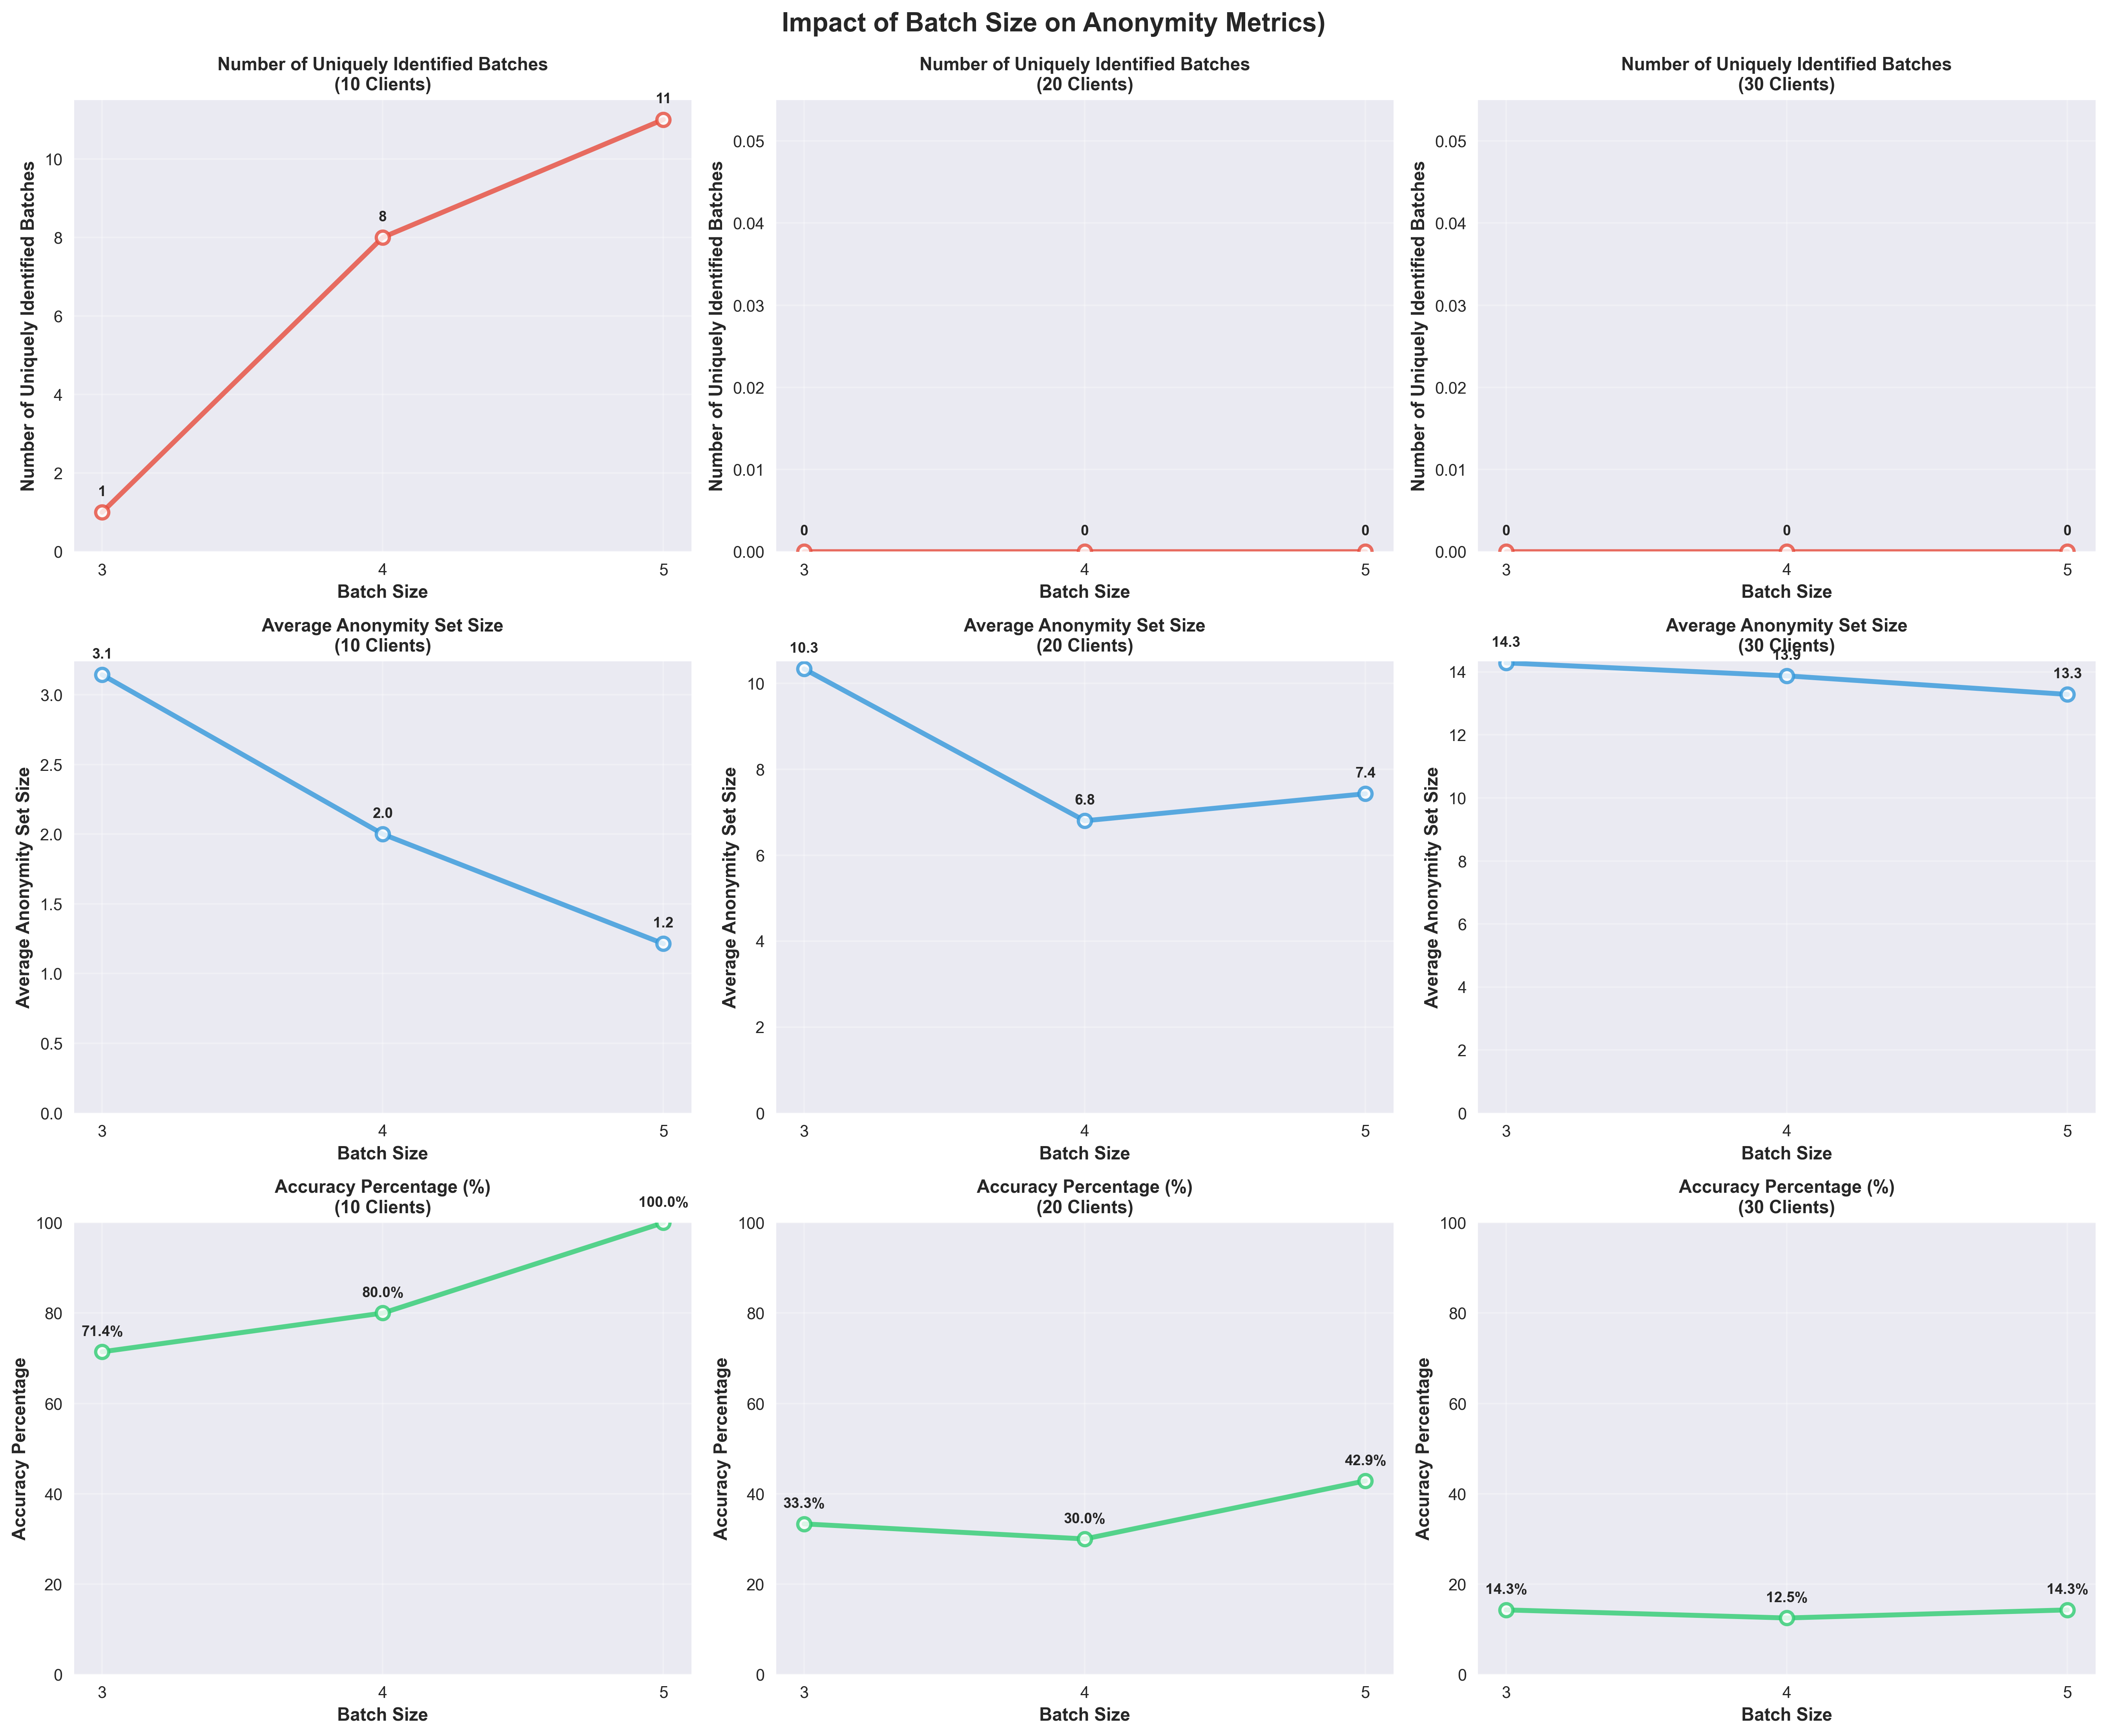
\includegraphics[width=\textwidth]{diagrams/batchsize_analysis.png}
% \caption{Impact of batch size on various anonymity metrics across different numbers of clients (10, 20, and 30 clients). The plots show how batch size affects the number of uniquely identified batches, average anonymity set size, and accuracy percentage.}
\label{fig:batchsize_analysis}
\end{figure*}

% \paragraph{Impact of Client Count on Anonymity Metrics}
% The simulation duration significantly impacts the anonymity characteristics of the mixnet system.

\begin{figure*}[!htb]
\centering
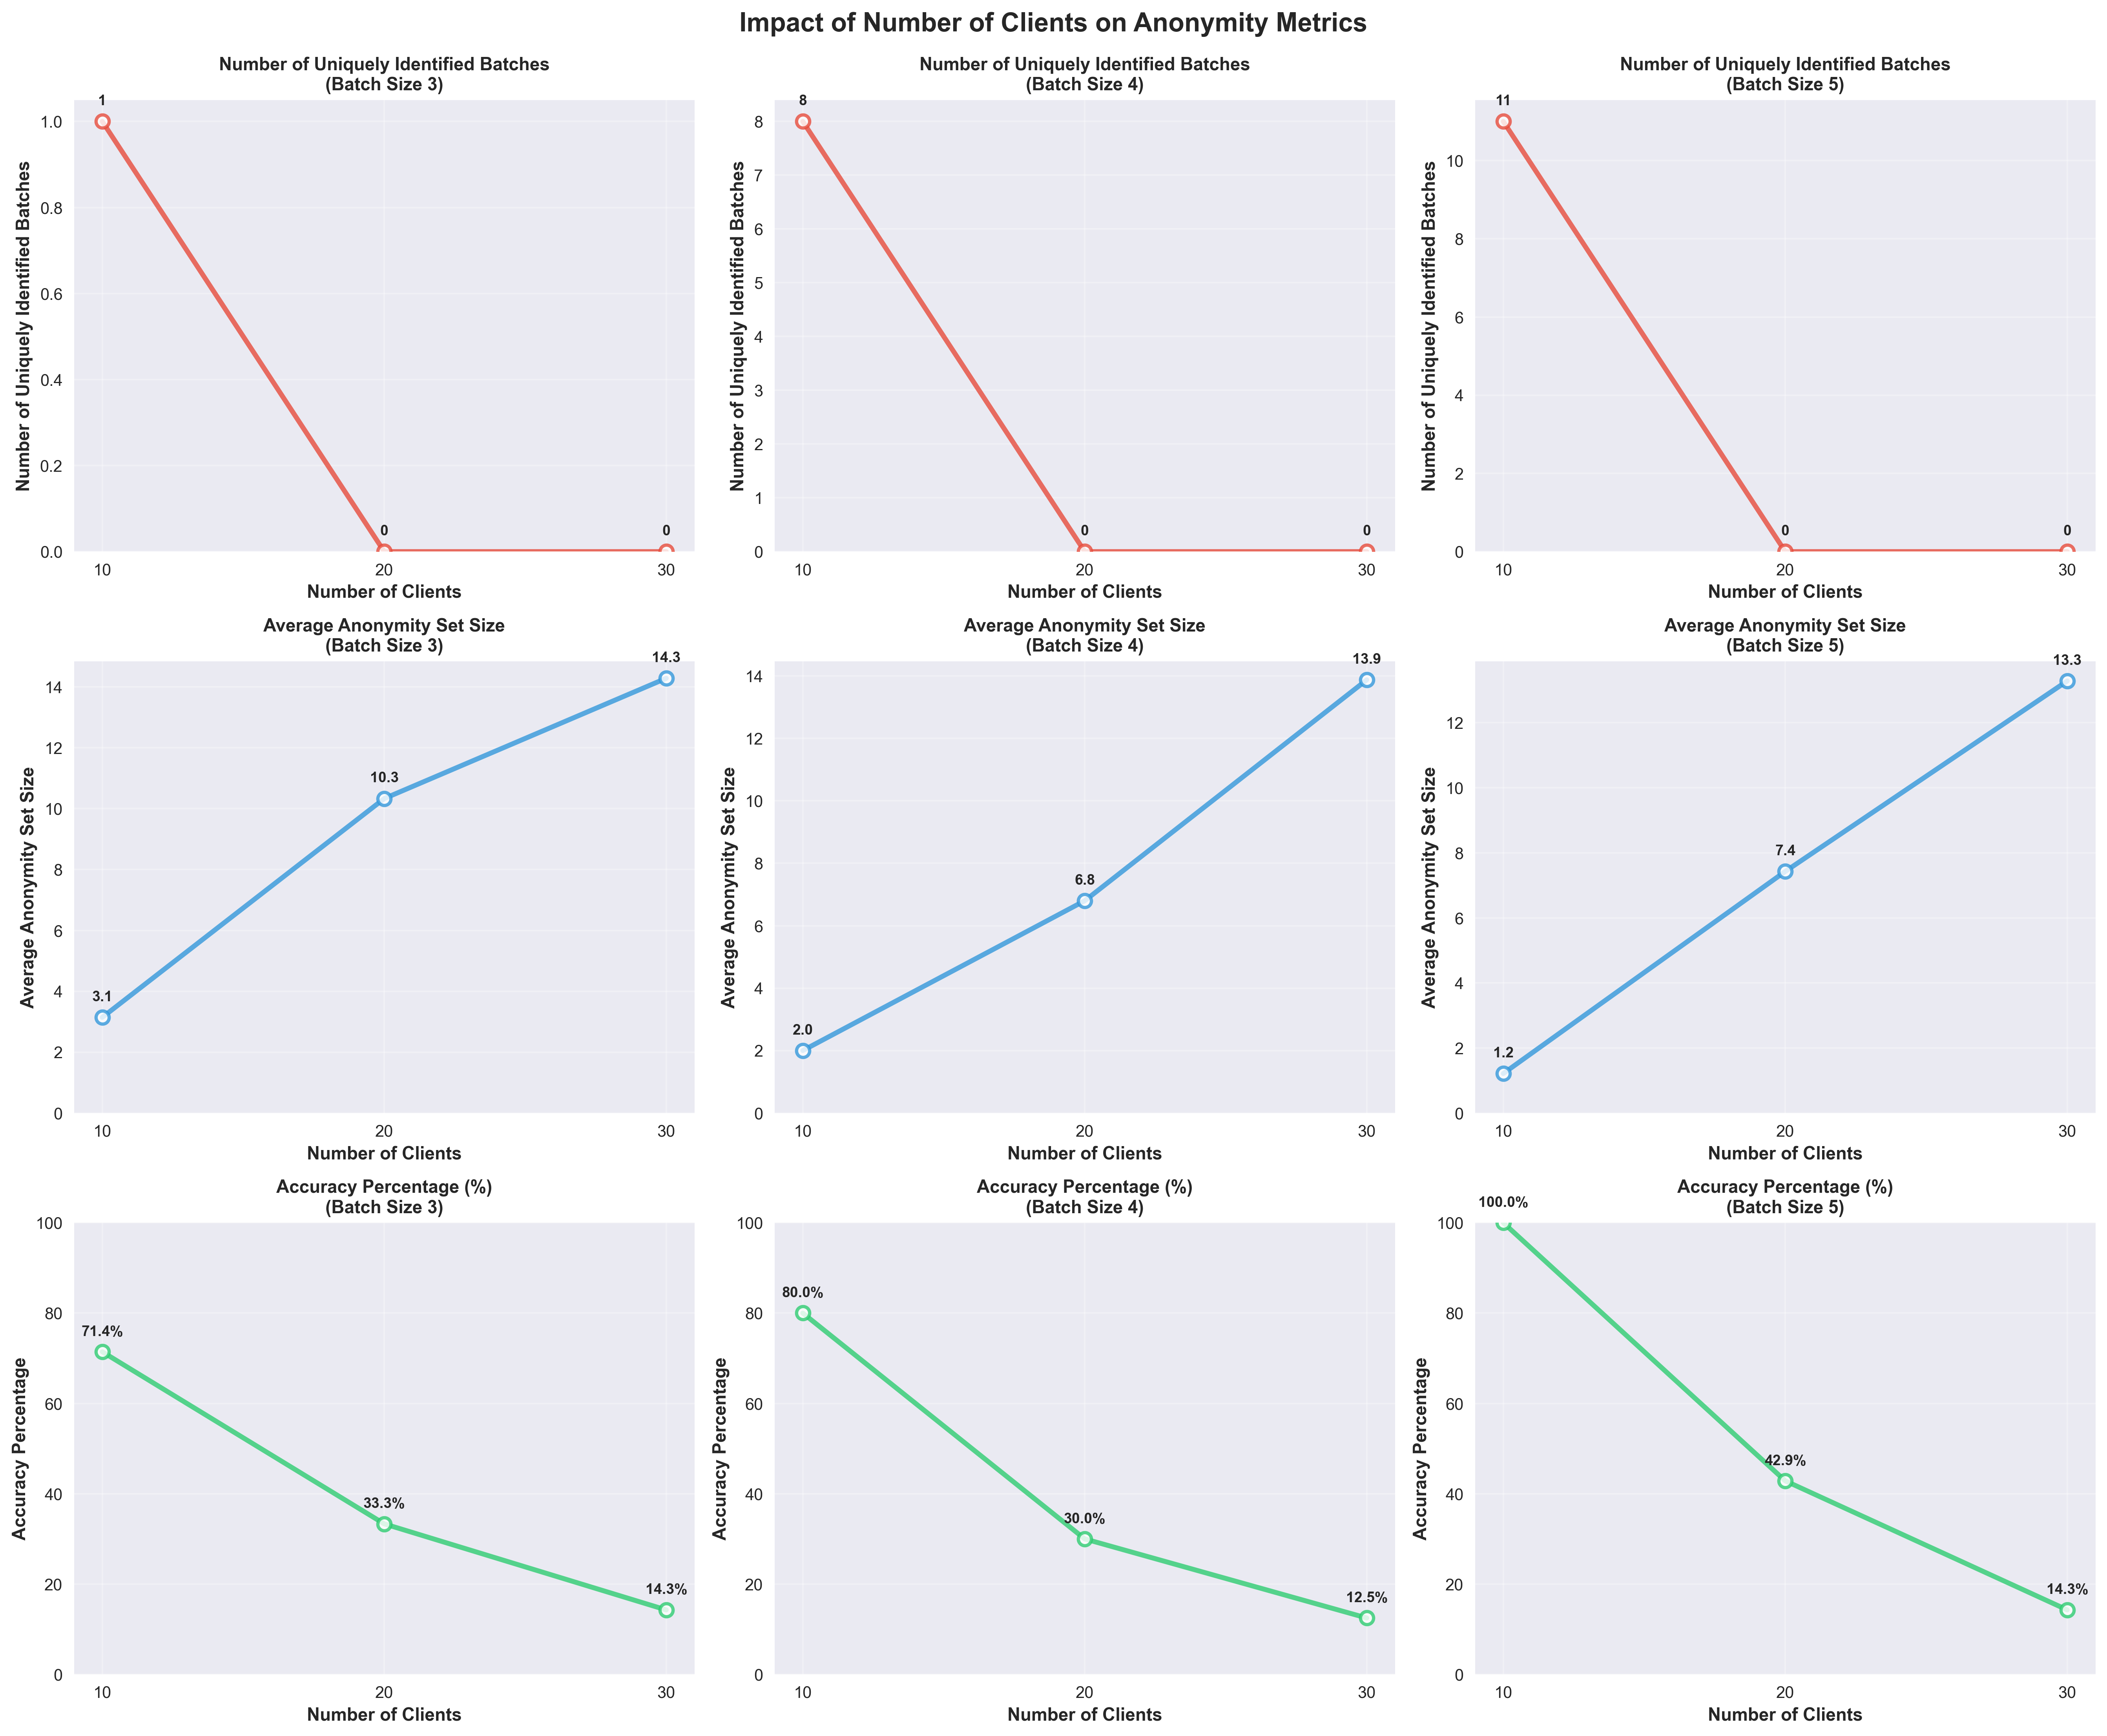
\includegraphics[width=\textwidth]{diagrams/client_analysis.png}
% \caption{Comparison of anonymity metrics for 12-hour (left) and 24-hour (right) simulation durations showing the effect of longer observation periods on batch correlation.}
\label{fig:client_analysis}
\end{figure*}

% \paragraph{Temporal Analysis}
% The number of clients in the system has a direct correlation with the achievable anonymity levels.

\begin{figure*}[!htb]
\centering
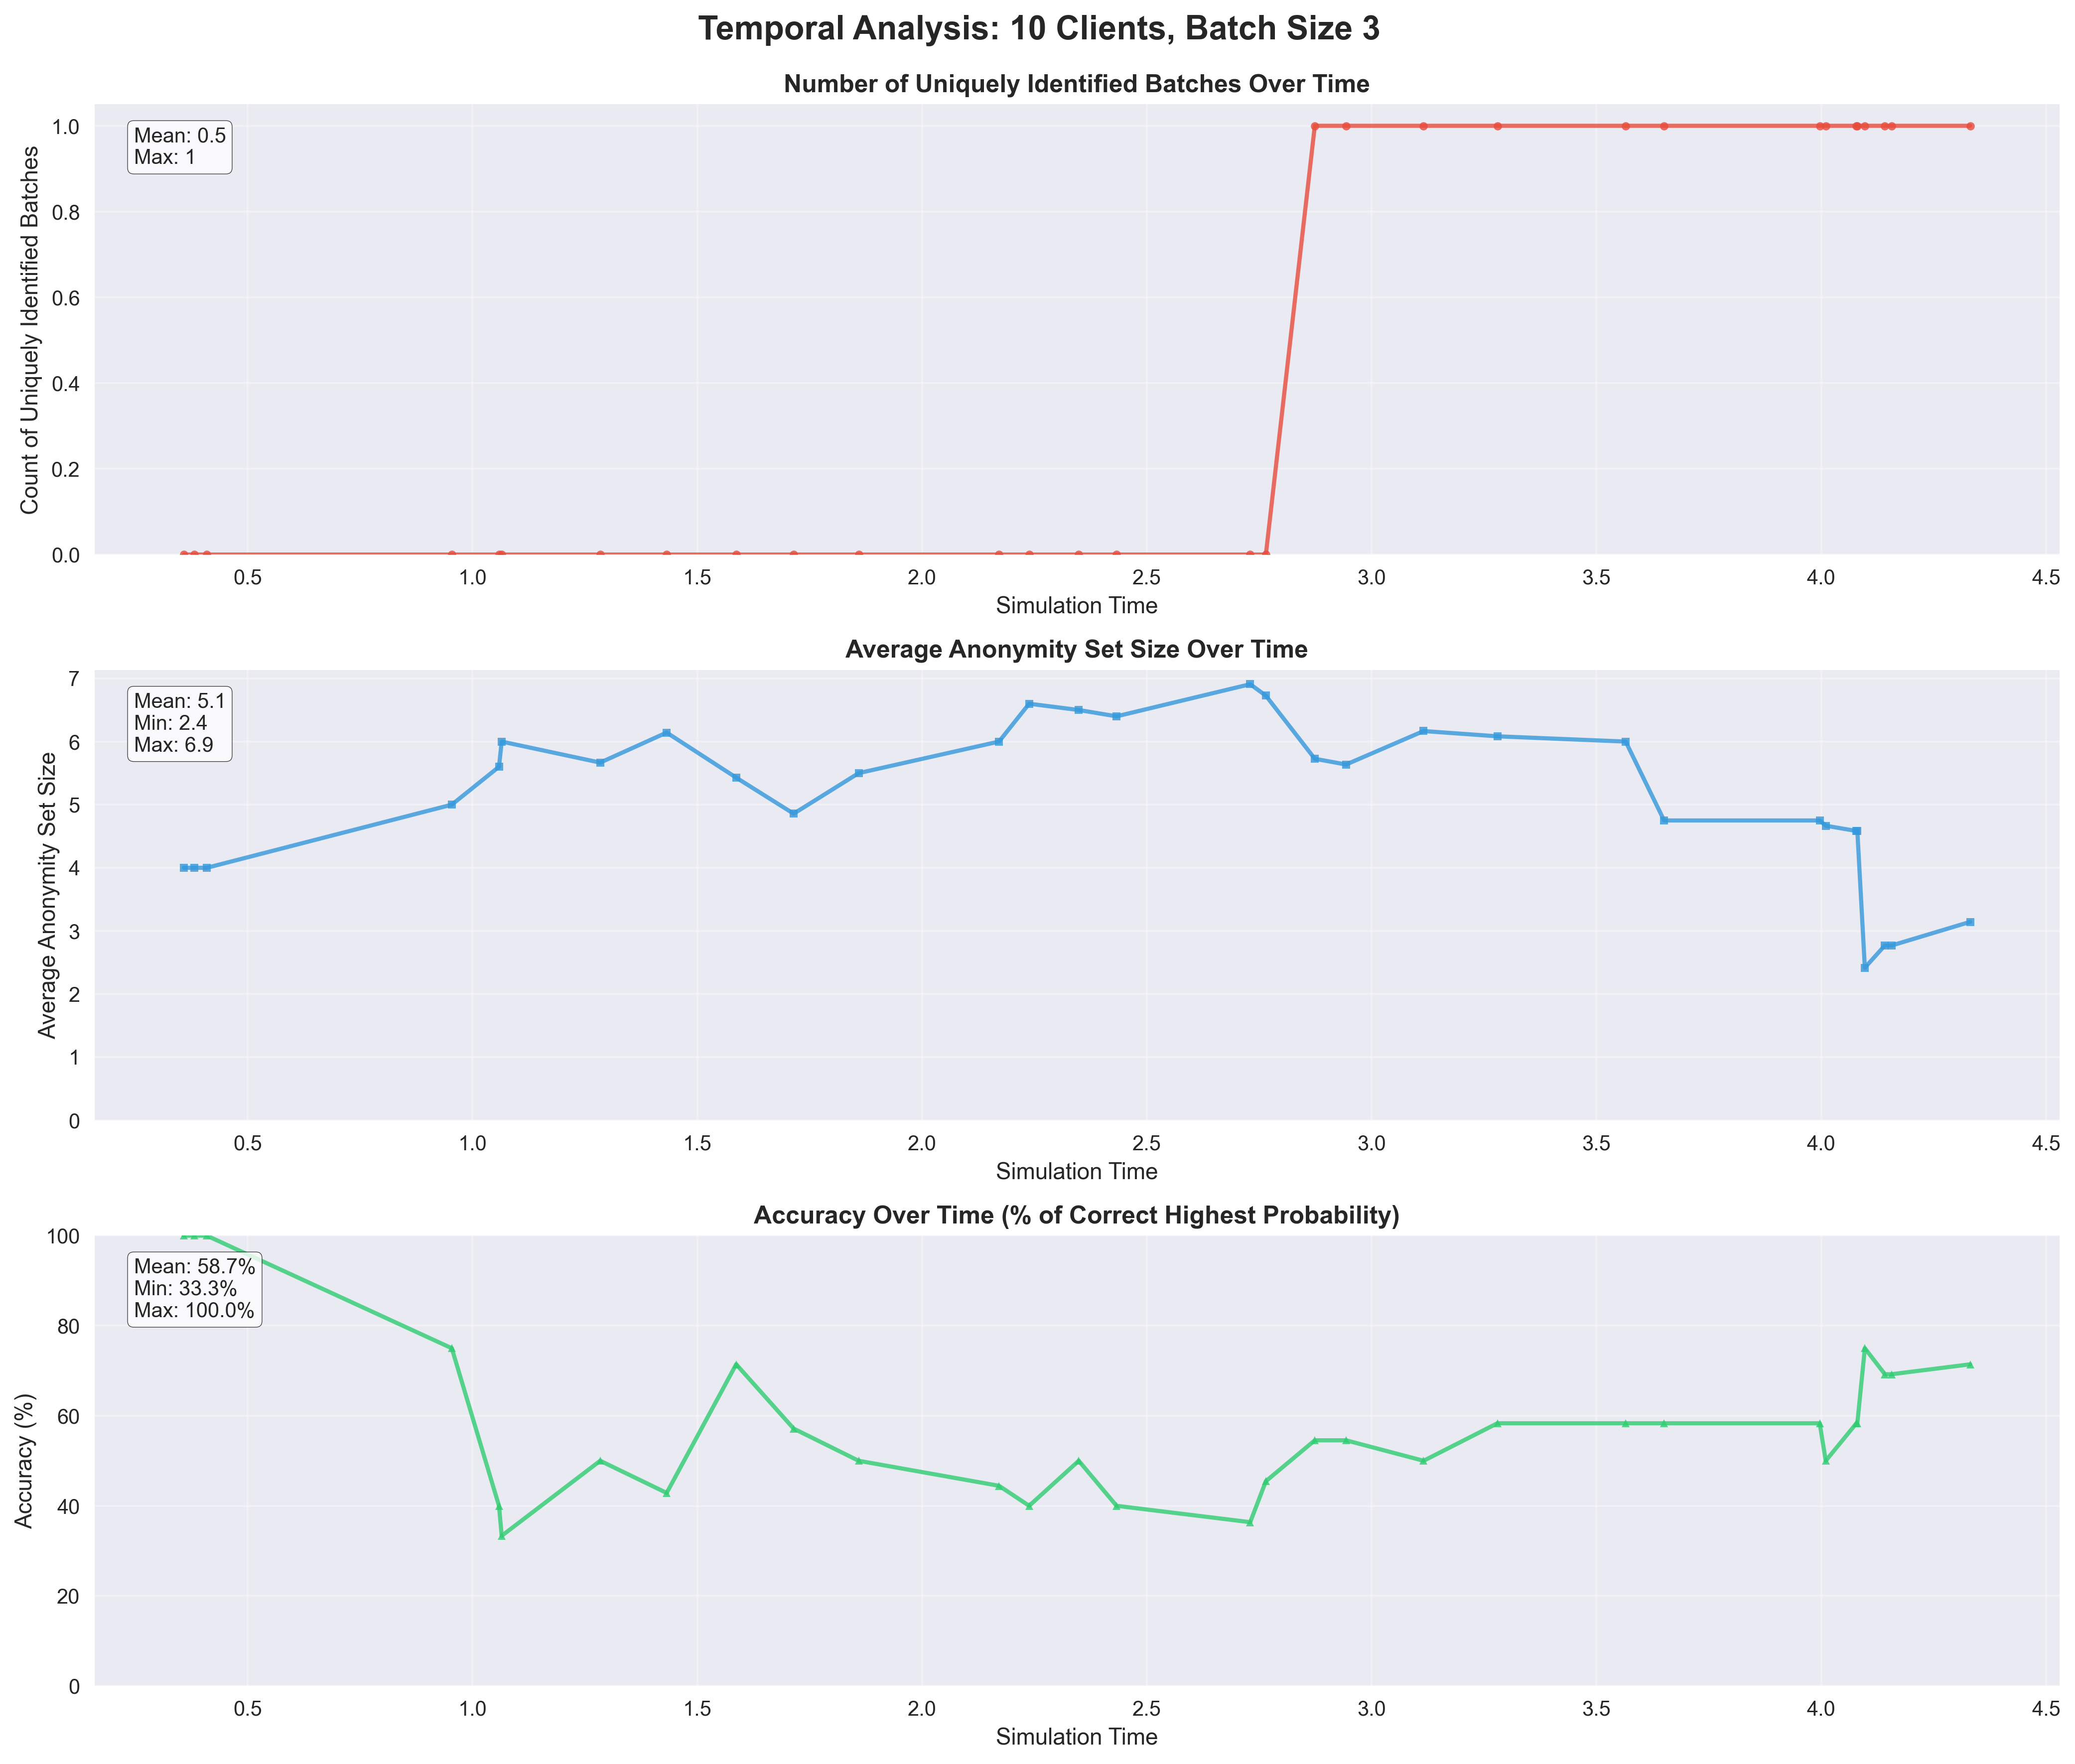
\includegraphics[width=\textwidth]{diagrams/temporal_analysis_10_3.png}
% \caption{Comparison of anonymity metrics for 12-hour (left) and 24-hour (right) simulation durations showing the effect of longer observation periods on batch correlation.}
\label{fig:temporal_analysis_10_3}
\end{figure*}

\begin{figure*}[!htb]
\centering
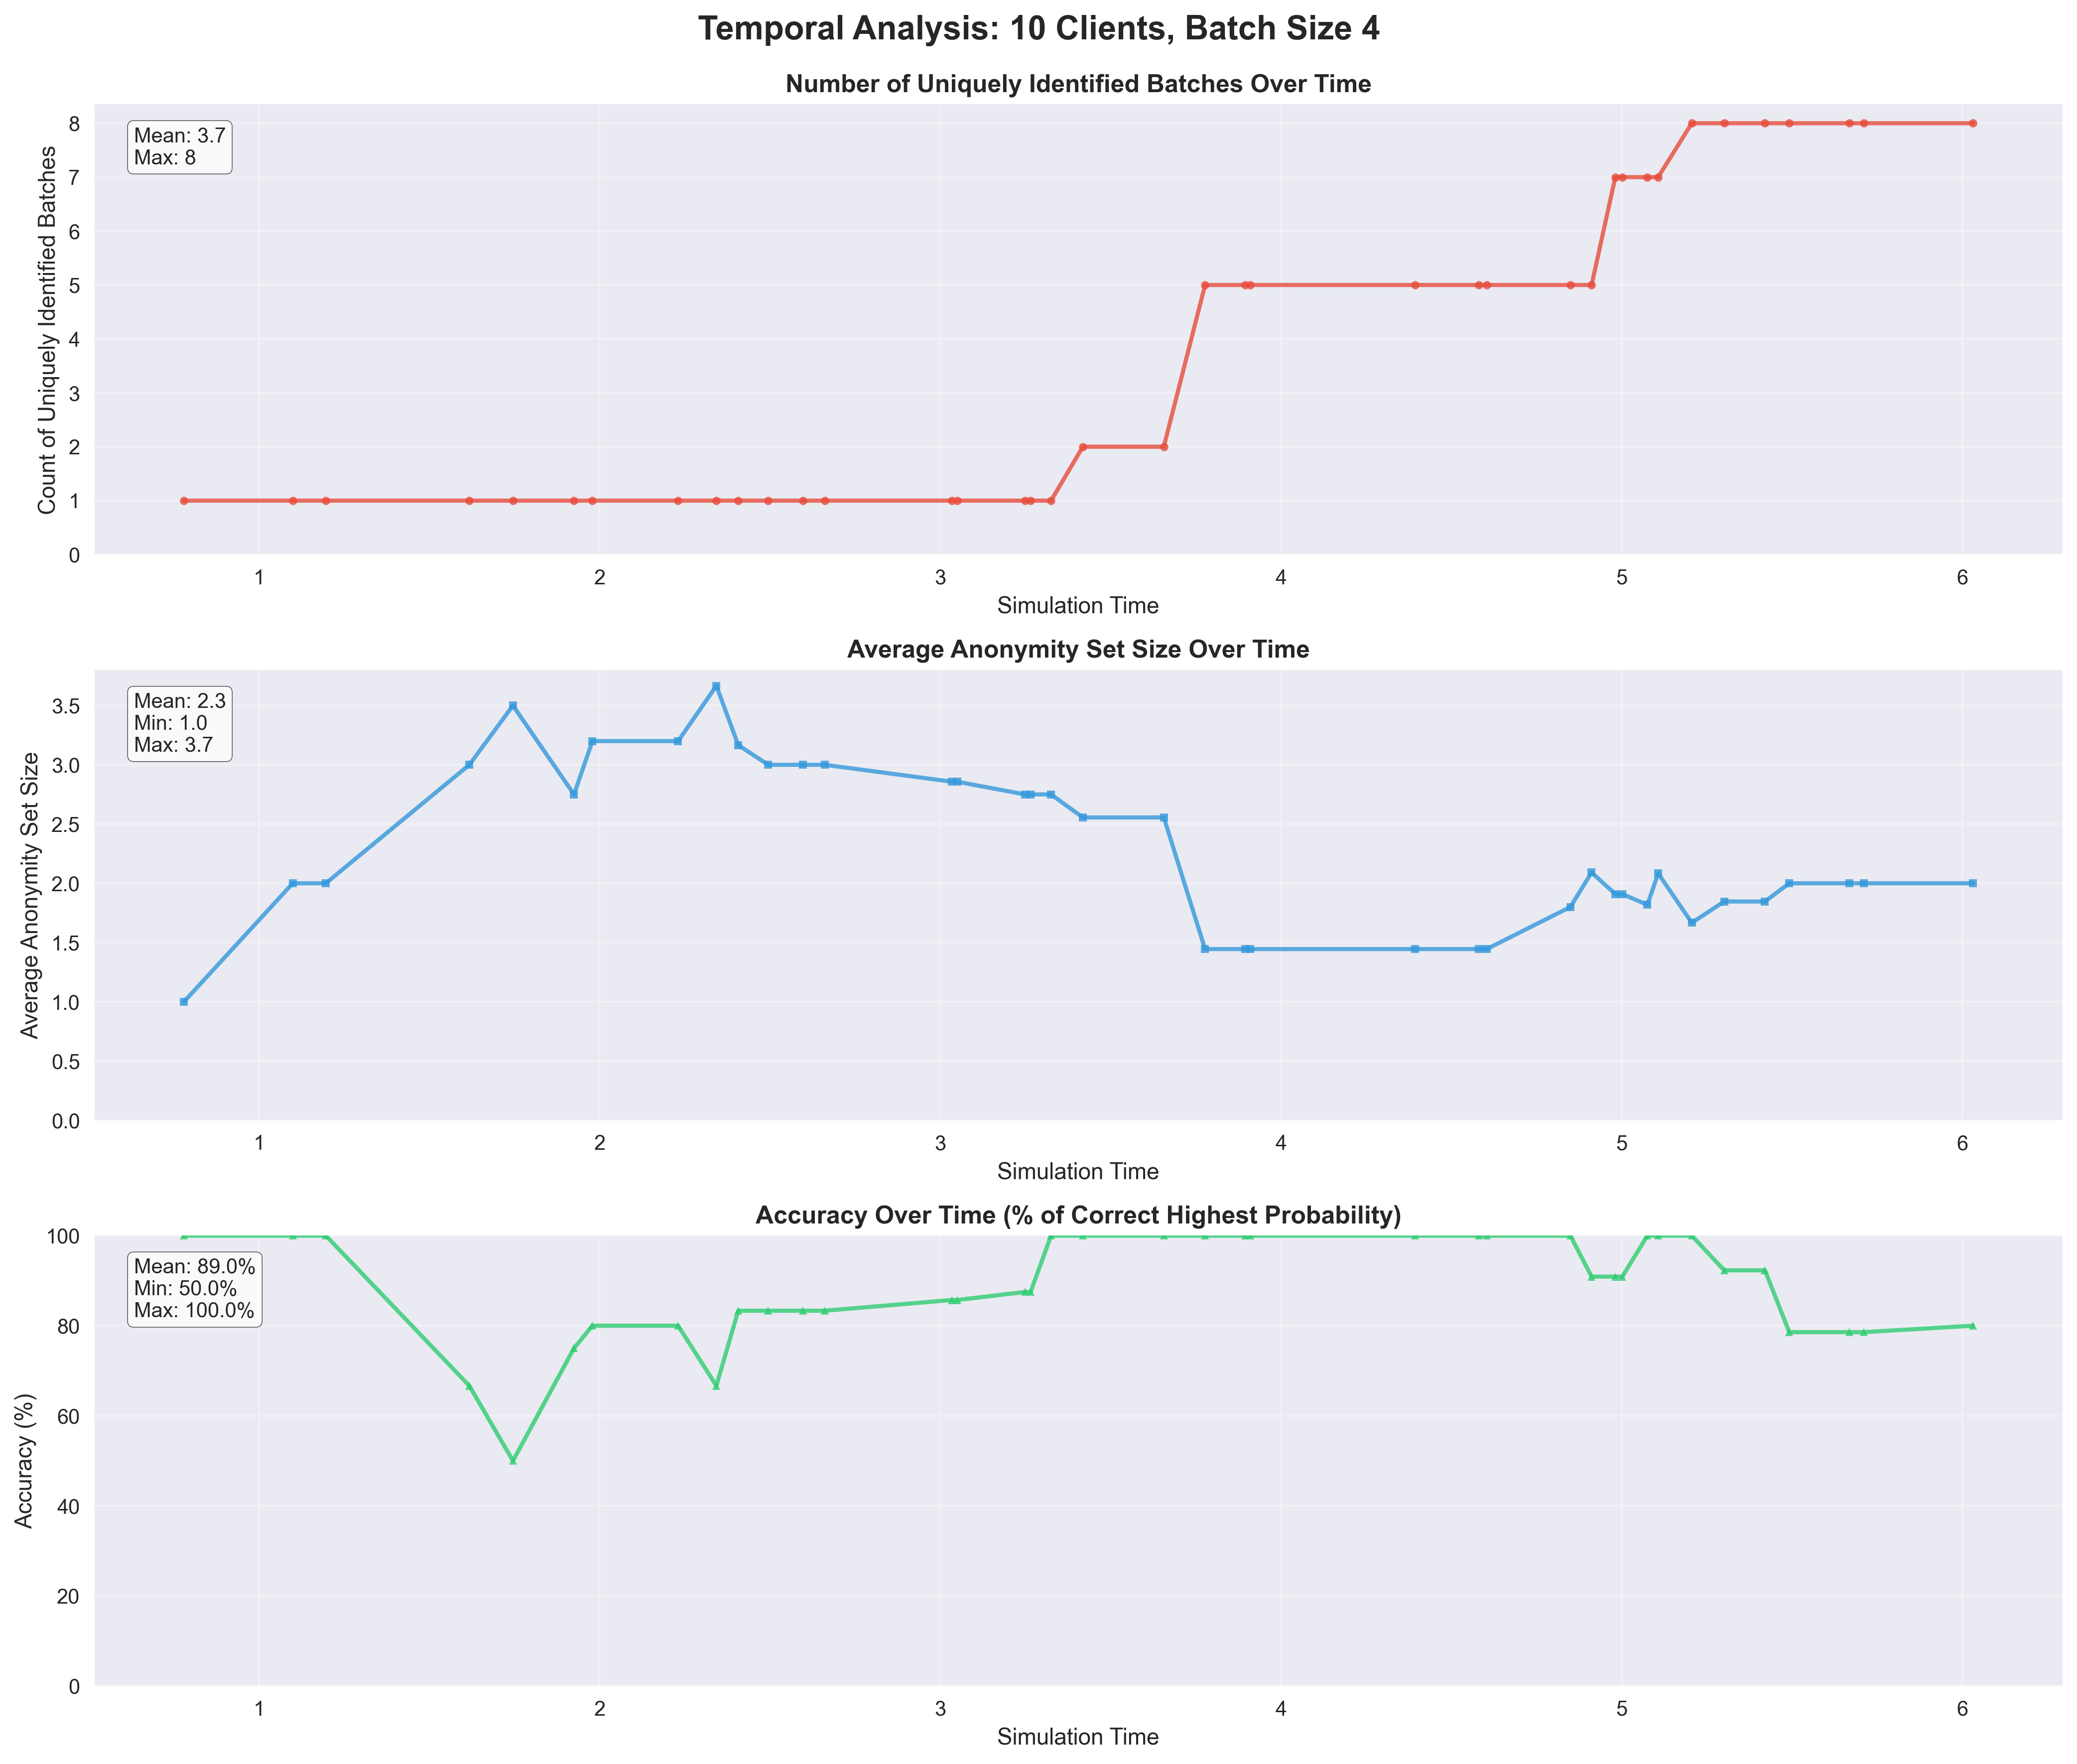
\includegraphics[width=\textwidth]{diagrams/temporal_analysis_10_4.png}
% \caption{Comparison of anonymity metrics for 12-hour (left) and 24-hour (right) simulation durations showing the effect of longer observation periods on batch correlation.}
\label{fig:temporal_analysis_10_4}
\end{figure*}

\begin{figure*}[!htb]
\centering
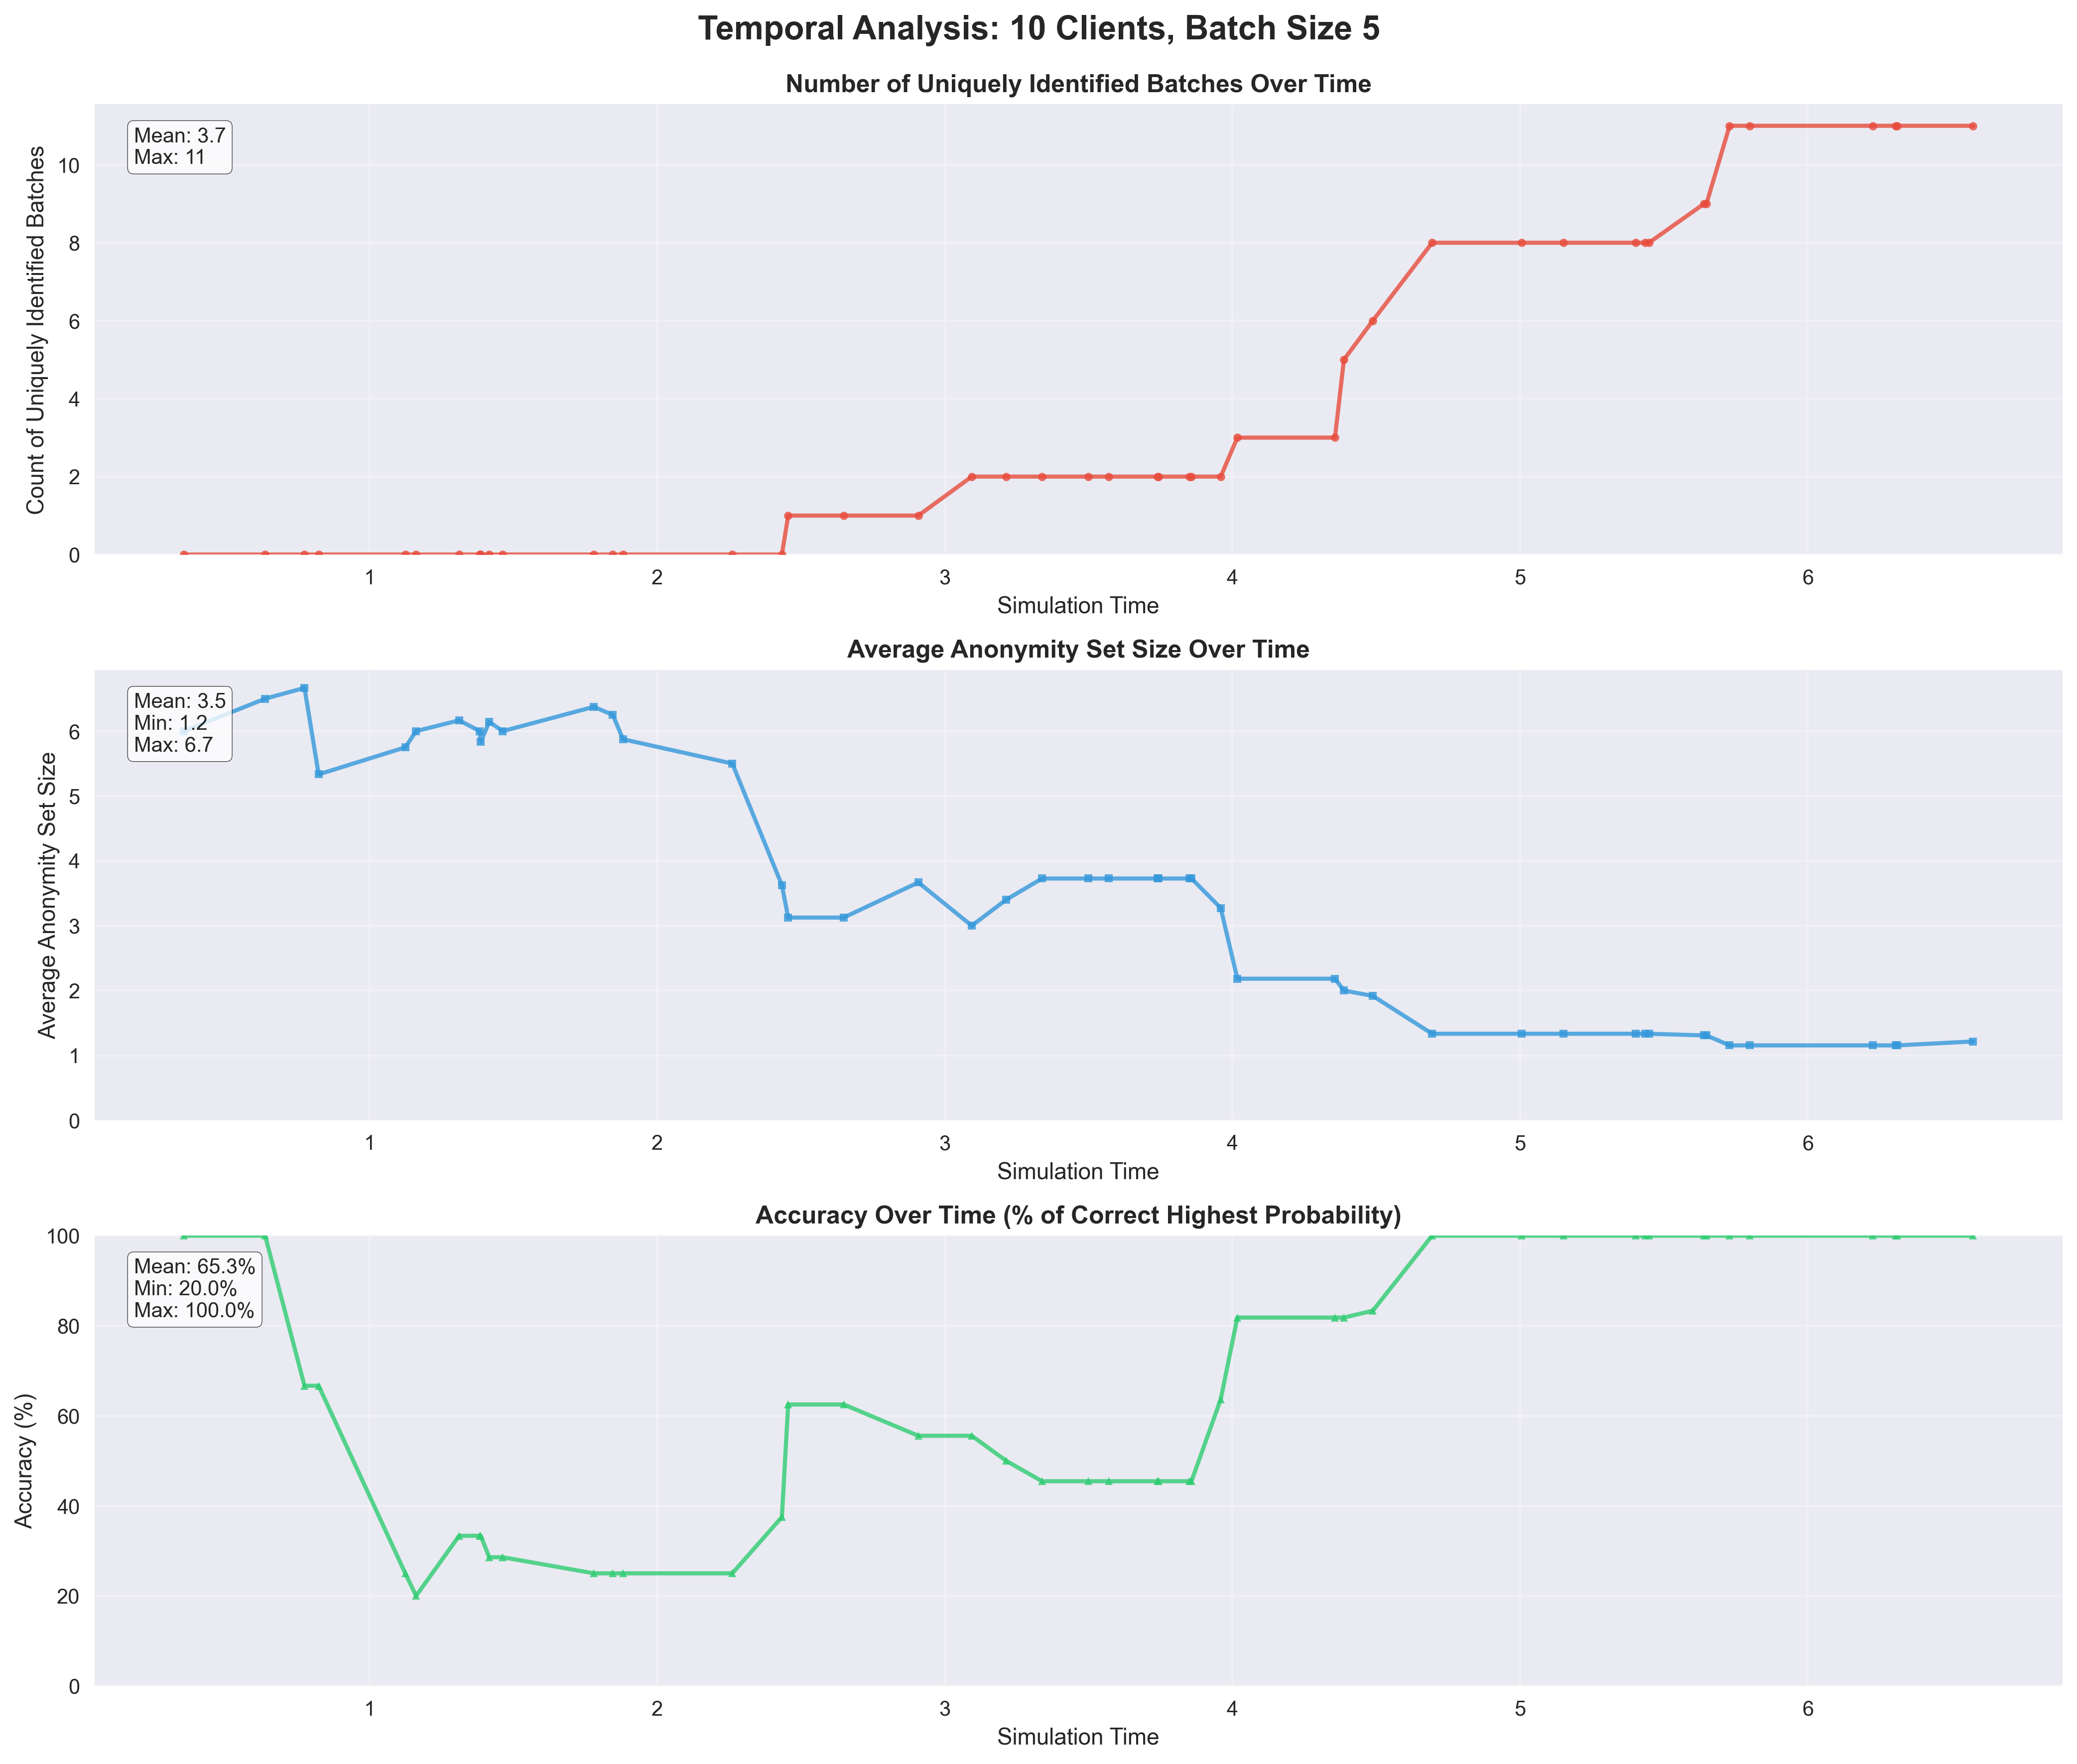
\includegraphics[width=\textwidth]{diagrams/temporal_analysis_10_5.png}
% \caption{Comparison of anonymity metrics for 12-hour (left) and 24-hour (right) simulation durations showing the effect of longer observation periods on batch correlation.}
\label{fig:temporal_analysis_10_5}
\end{figure*}

\begin{figure*}[!htb]
\centering
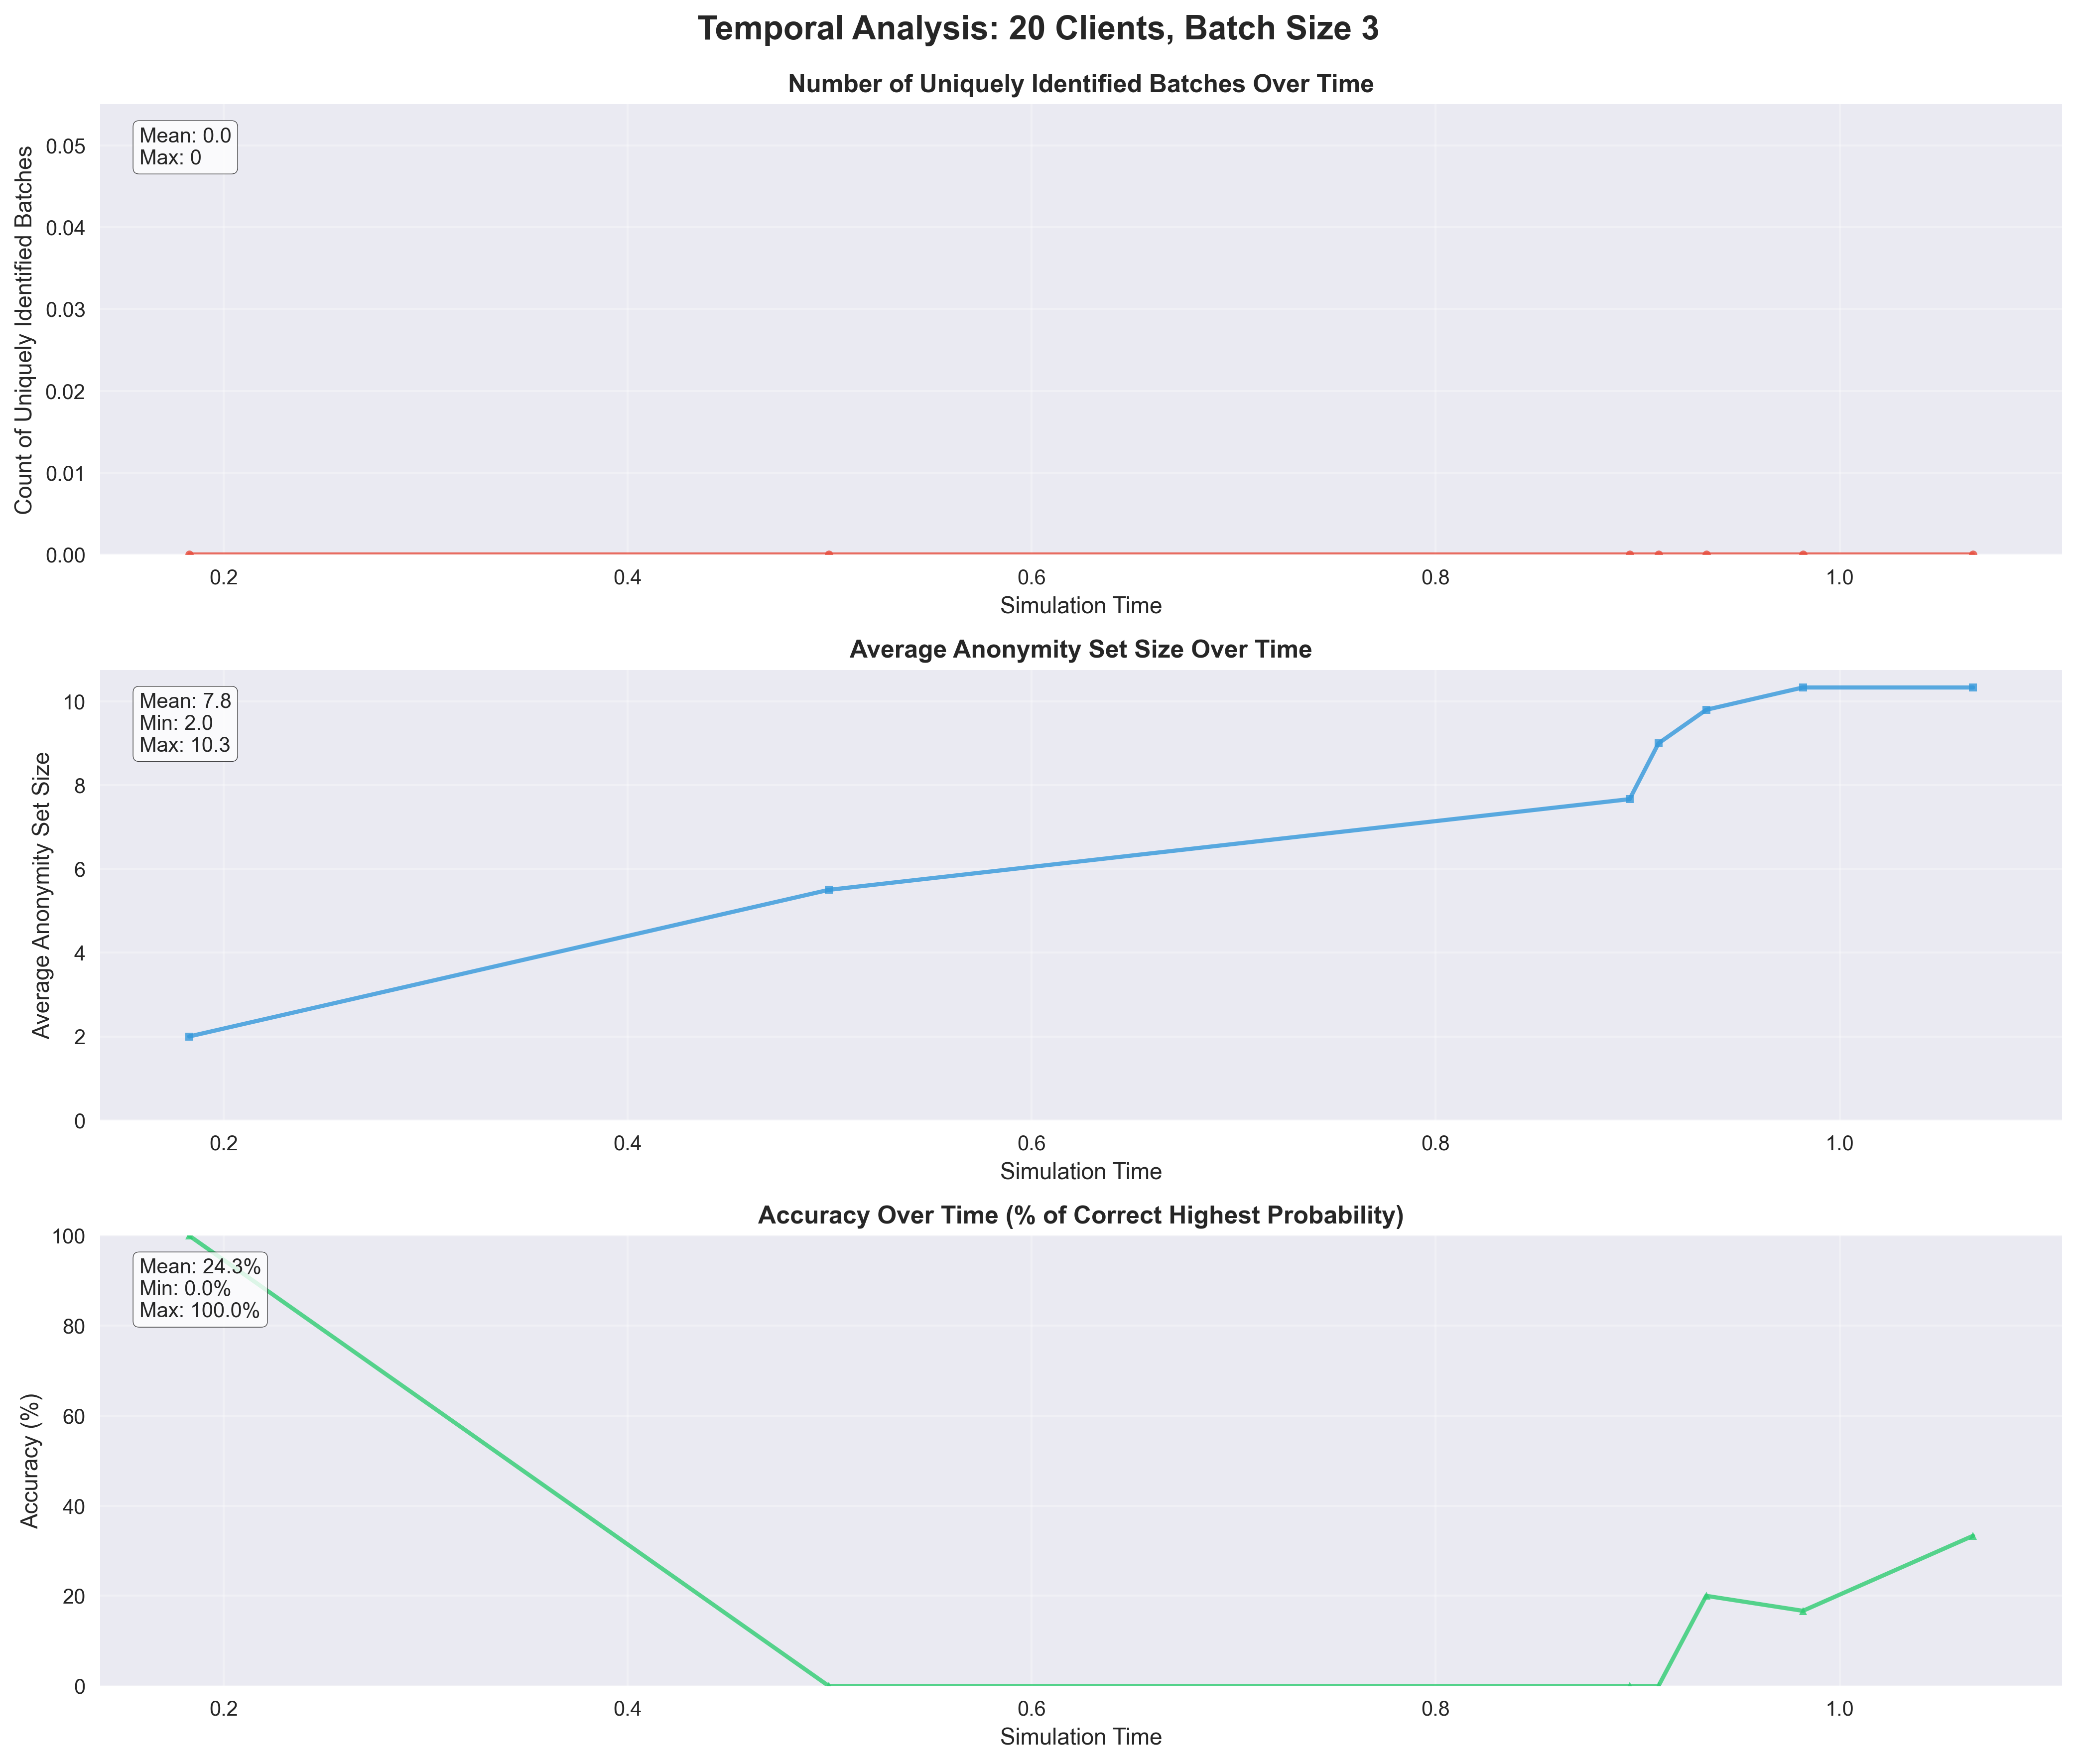
\includegraphics[width=\textwidth]{diagrams/temporal_analysis_20_3.png}
% \caption{Comparison of anonymity metrics for 12-hour (left) and 24-hour (right) simulation durations showing the effect of longer observation periods on batch correlation.}
\label{fig:temporal_analysis_20_3}
\end{figure*}

\begin{figure*}[!htb]
\centering
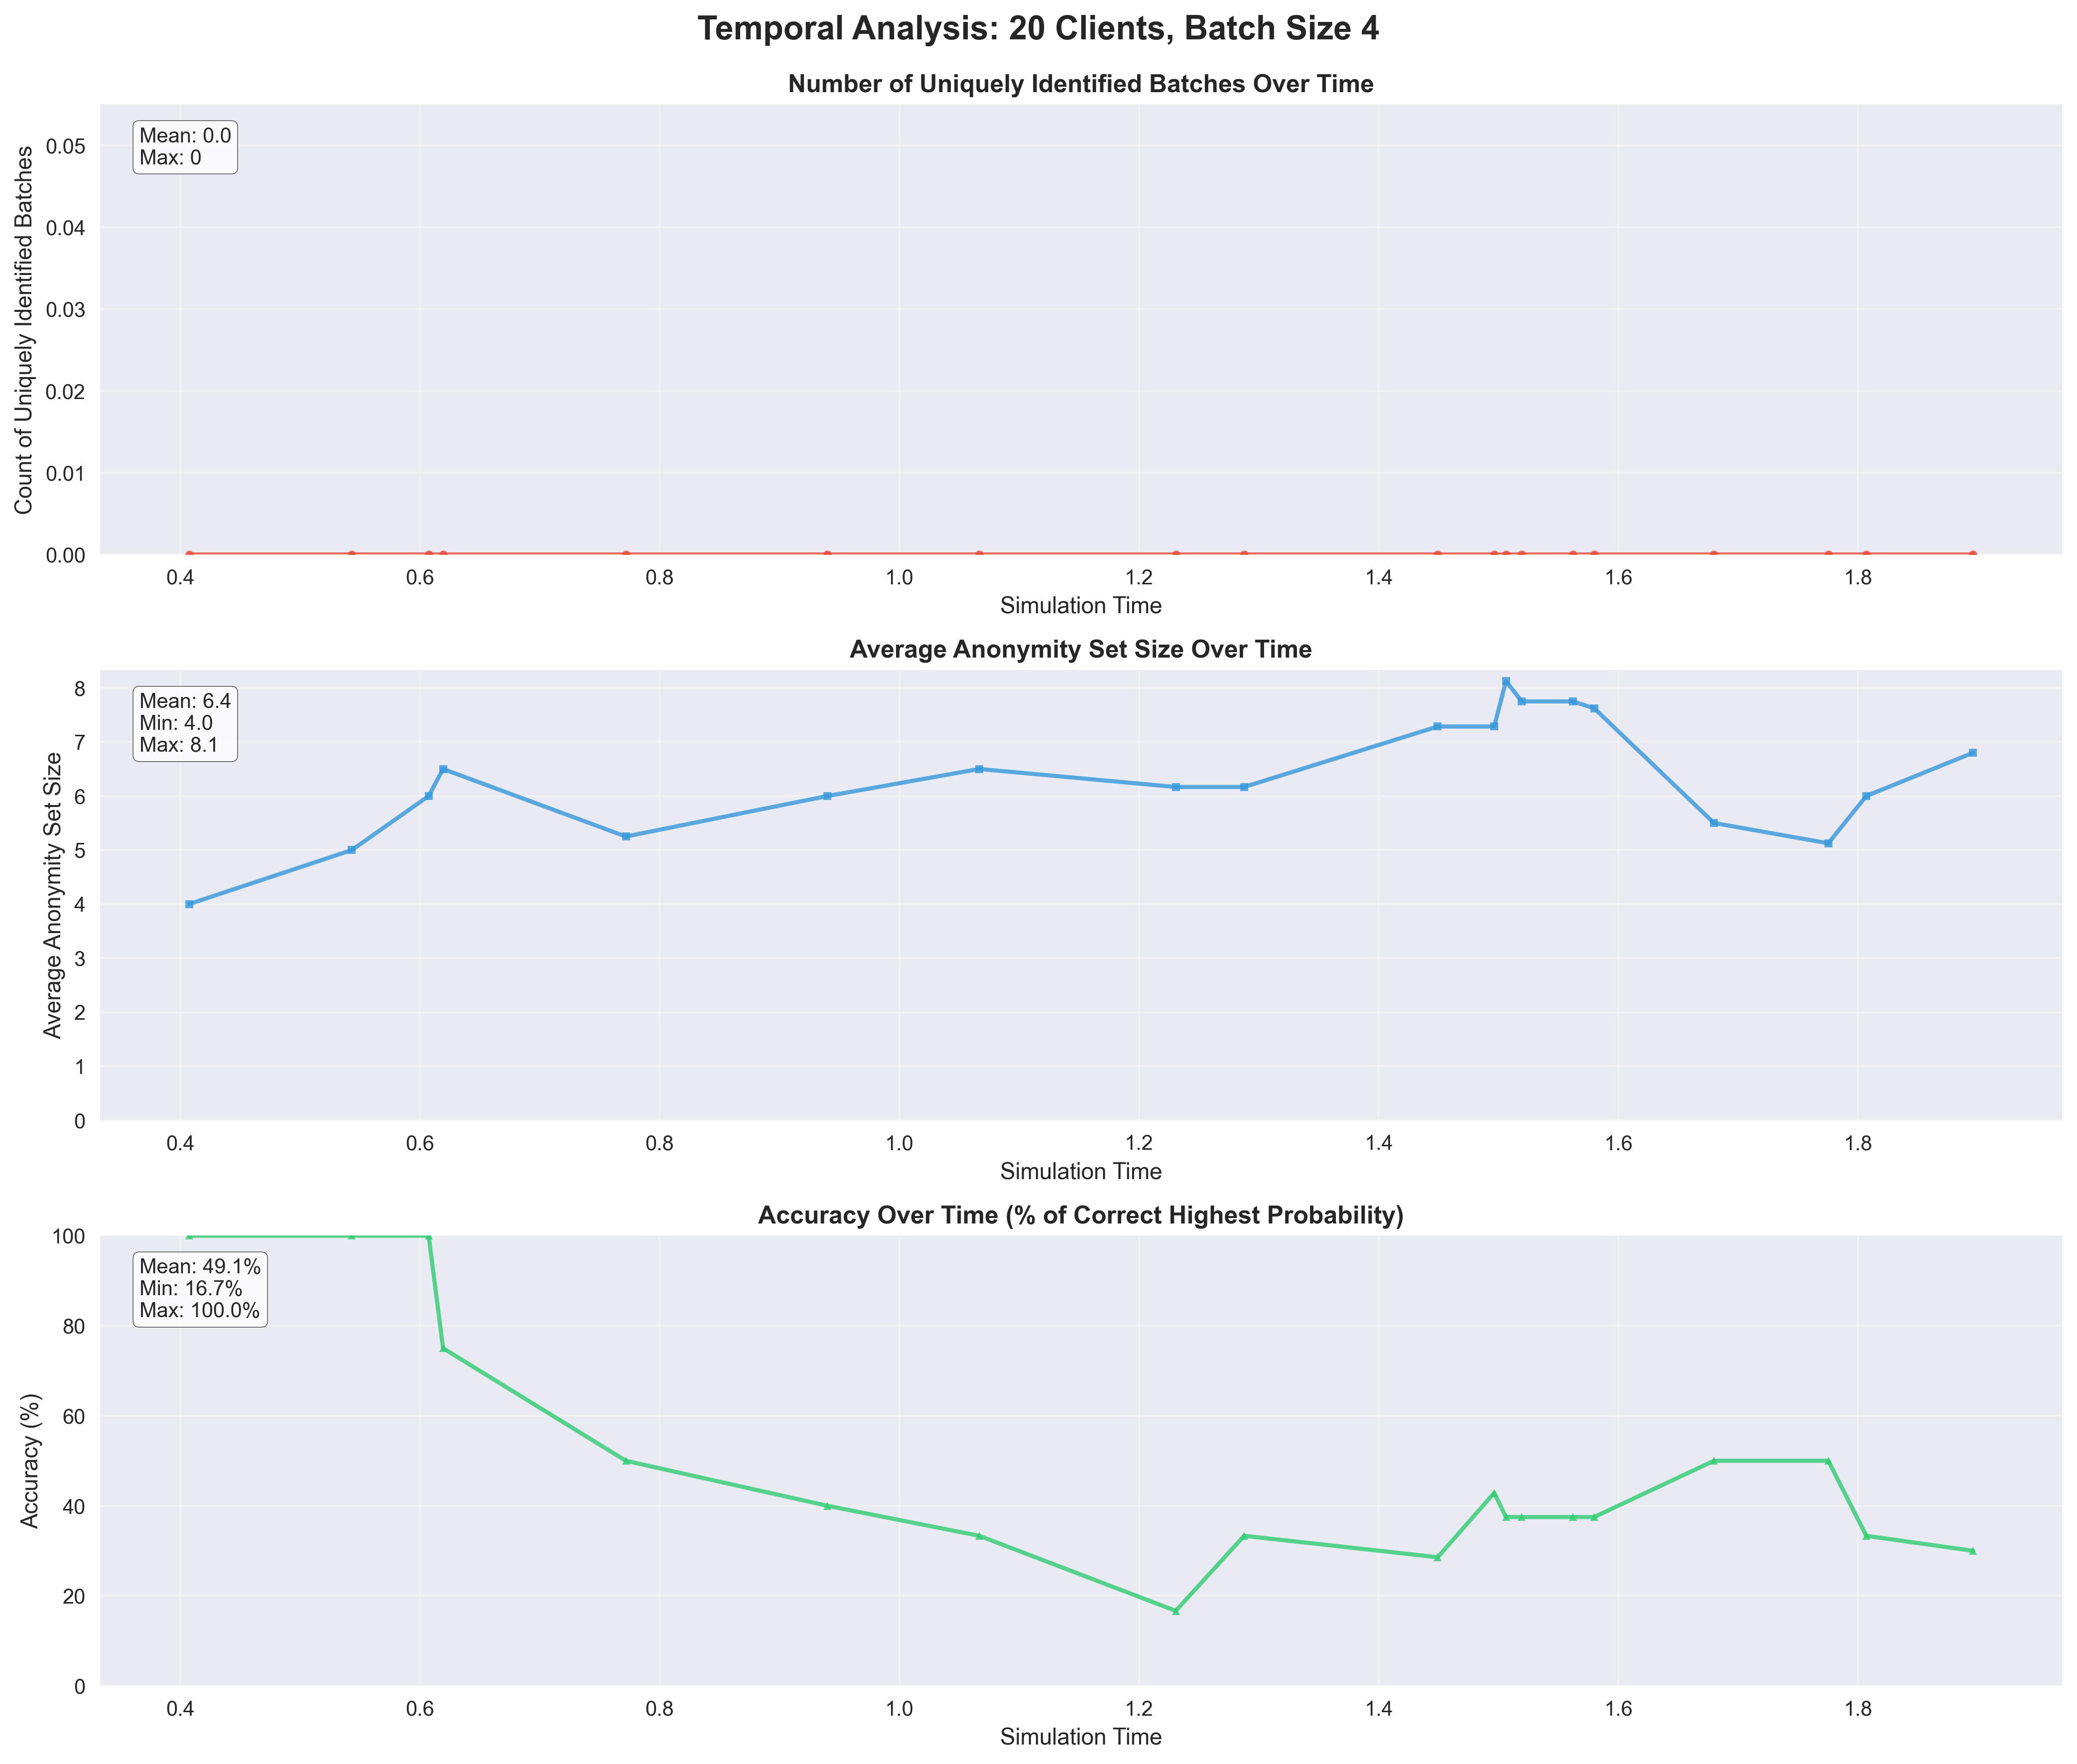
\includegraphics[width=\textwidth]{diagrams/temporal_analysis_20_4.png}
% \caption{Comparison of anonymity metrics for 12-hour (left) and 24-hour (right) simulation durations showing the effect of longer observation periods on batch correlation.}
\label{fig:temporal_analysis_20_4}
\end{figure*}

\begin{figure*}[!htb]
\centering
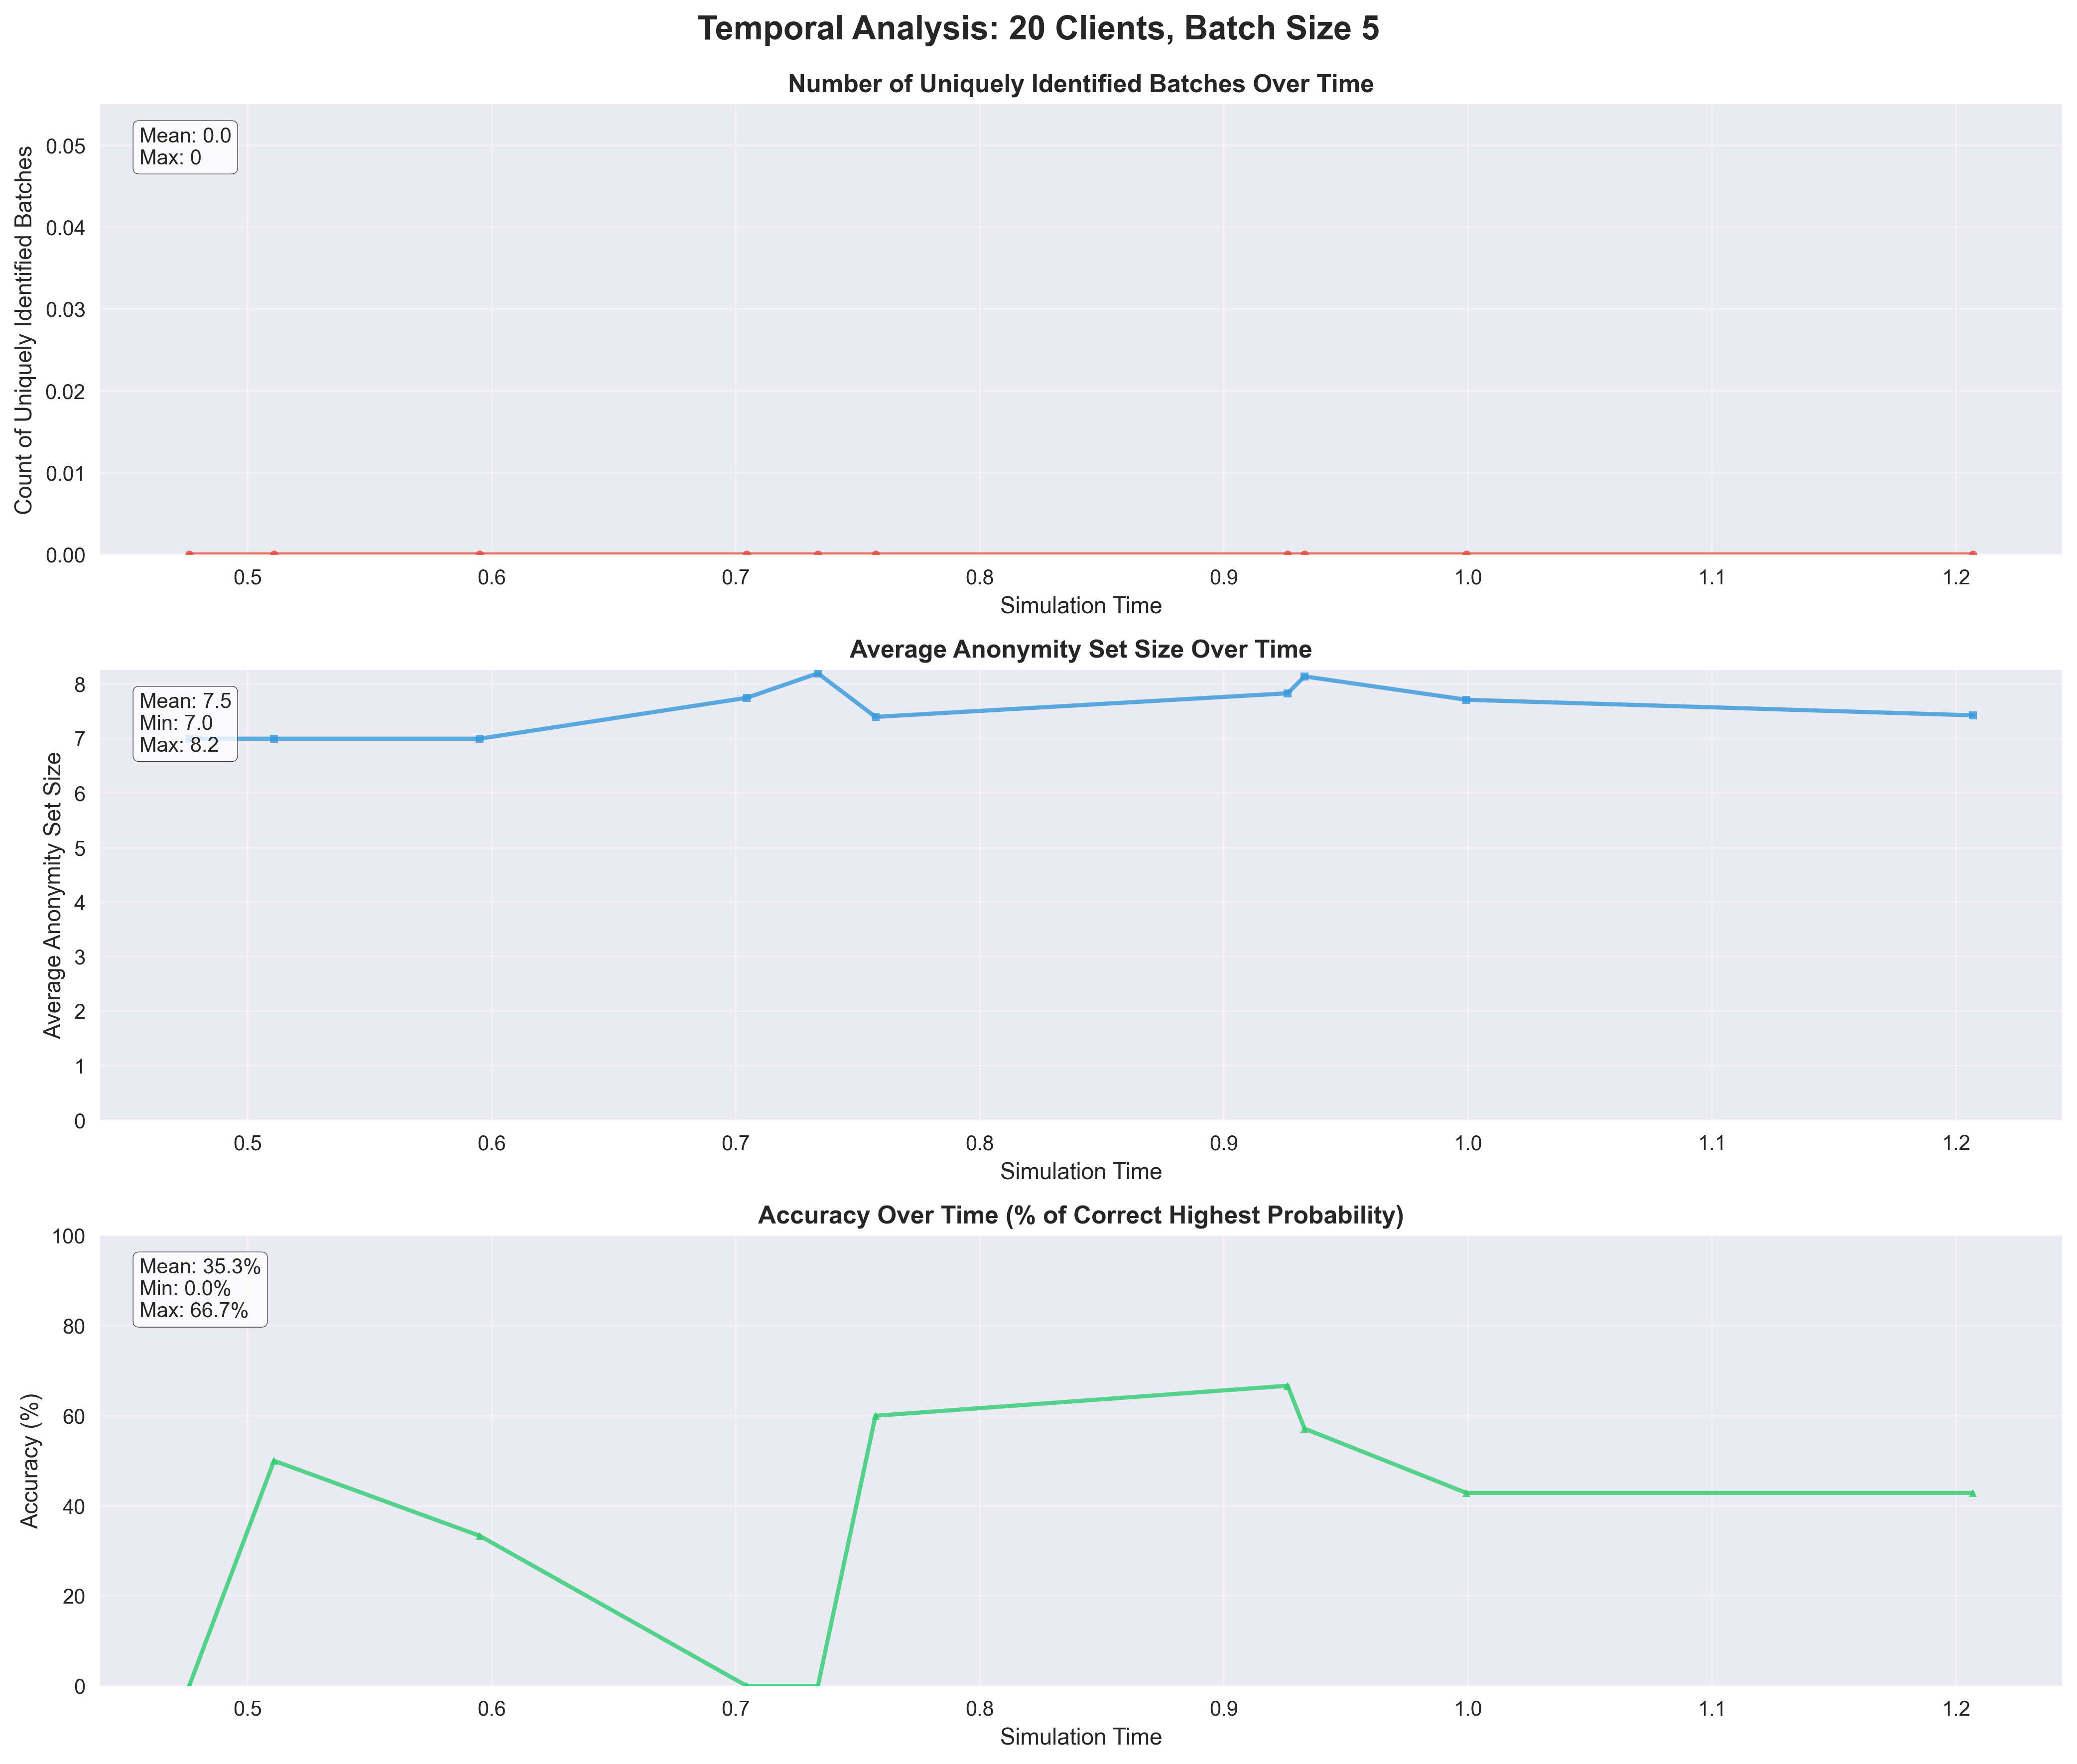
\includegraphics[width=\textwidth]{diagrams/temporal_analysis_20_5.png}
% \caption{Comparison of anonymity metrics for 12-hour (left) and 24-hour (right) simulation durations showing the effect of longer observation periods on batch correlation.}
\label{fig:temporal_analysis_20_5}
\end{figure*}

\begin{figure*}[!htb]
\centering
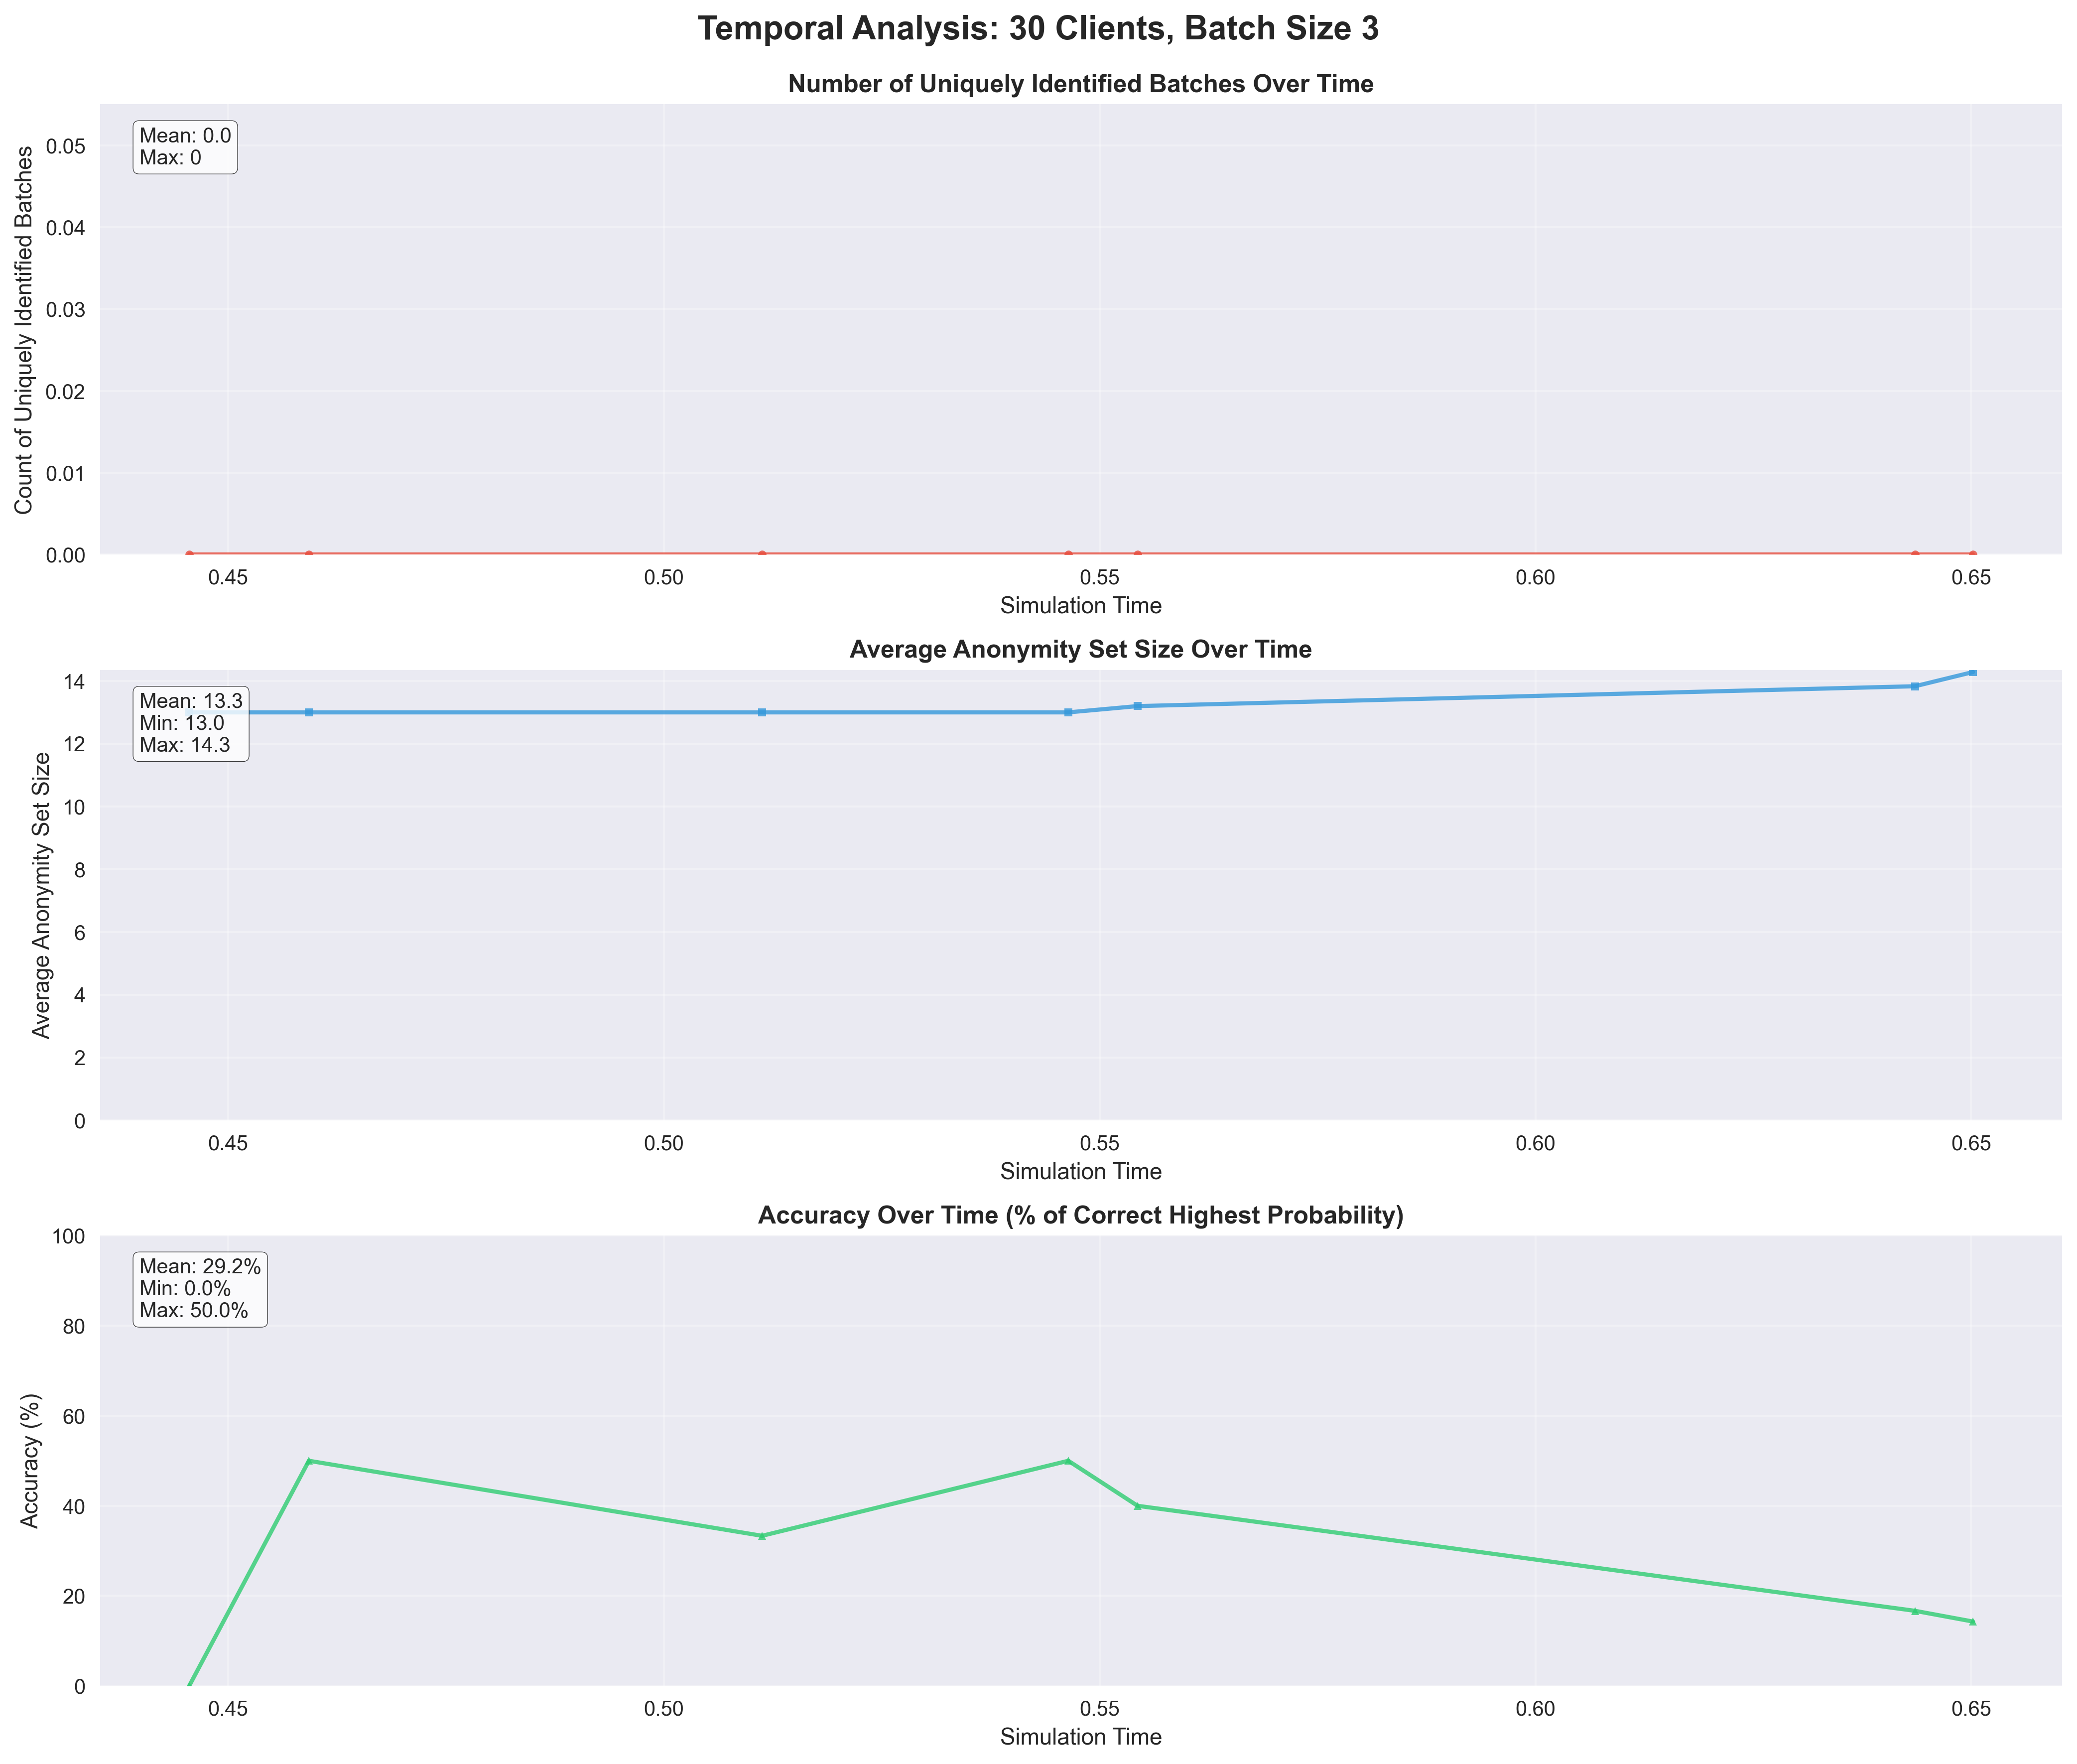
\includegraphics[width=\textwidth]{diagrams/temporal_analysis_30_3.png}
% \caption{Comparison of anonymity metrics for 12-hour (left) and 24-hour (right) simulation durations showing the effect of longer observation periods on batch correlation.}
\label{fig:temporal_analysis_30_3}
\end{figure*}

\begin{figure*}[!htb]
\centering
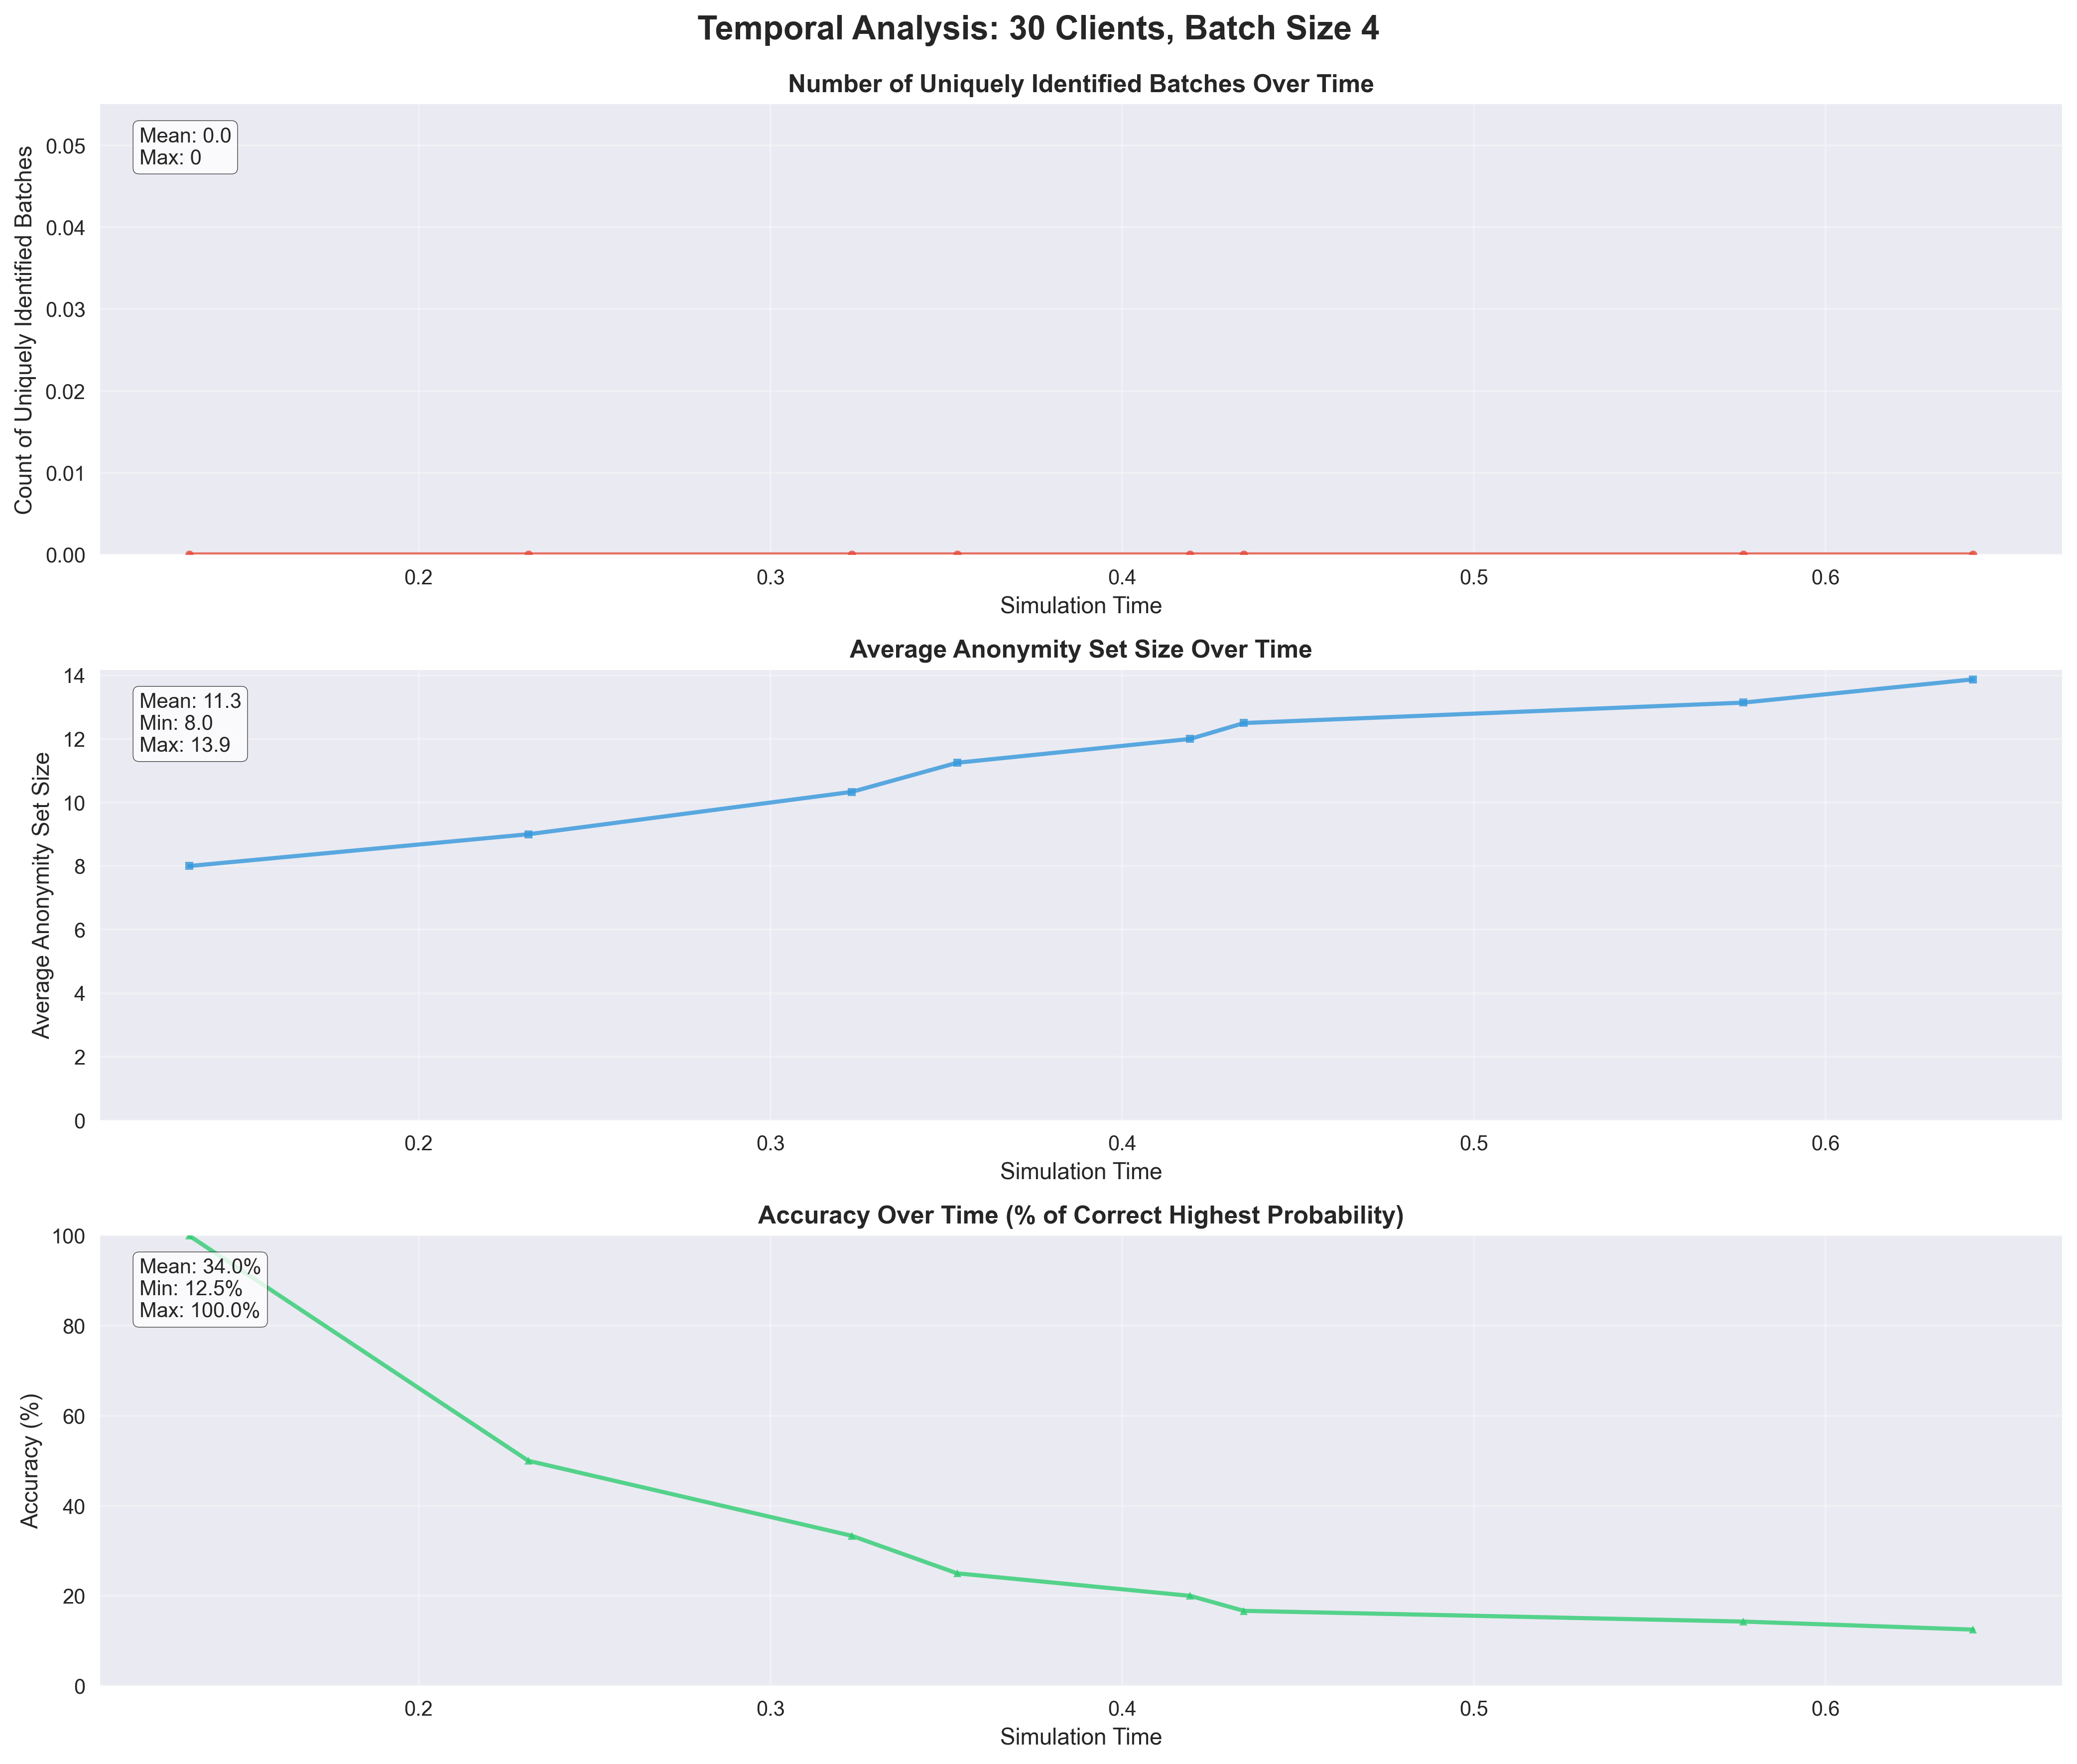
\includegraphics[width=\textwidth]{diagrams/temporal_analysis_30_4.png}
% \caption{Comparison of anonymity metrics for 12-hour (left) and 24-hour (right) simulation durations showing the effect of longer observation periods on batch correlation.}
\label{fig:temporal_analysis_30_4}
\end{figure*}

\begin{figure*}[!htb]
\centering
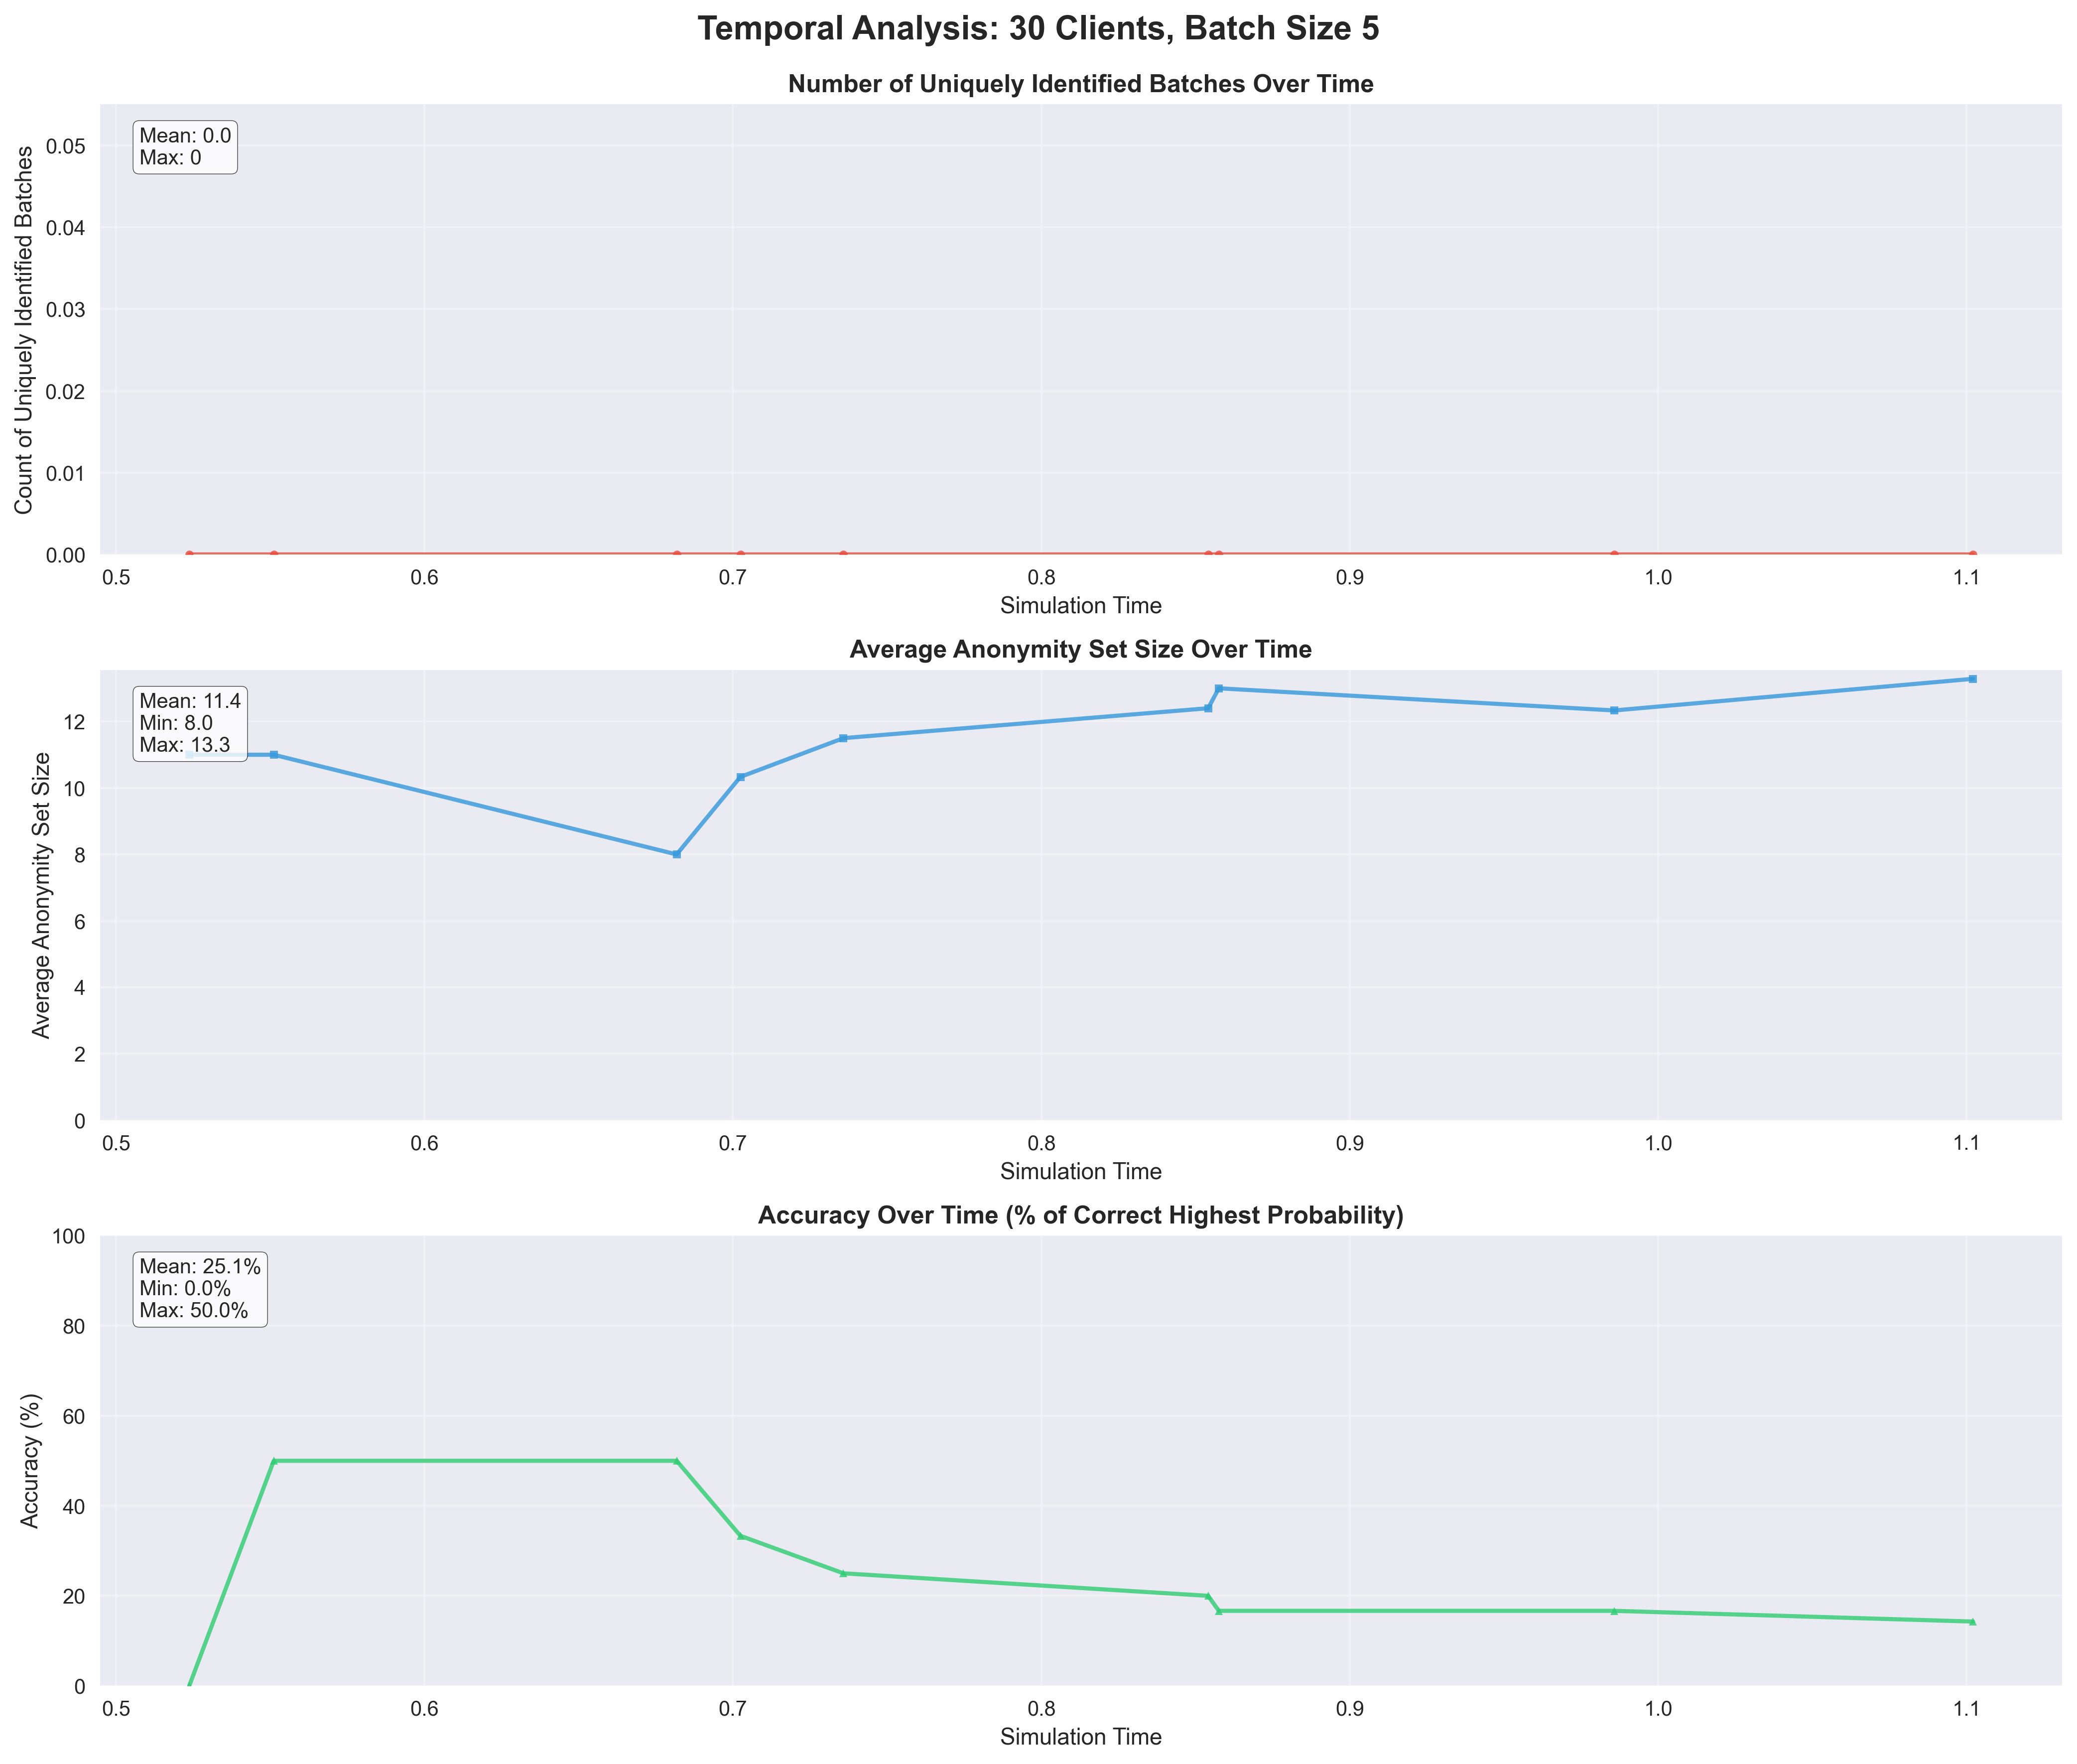
\includegraphics[width=\textwidth]{diagrams/temporal_analysis_30_5.png}
% \caption{Comparison of anonymity metrics for 12-hour (left) and 24-hour (right) simulation durations showing the effect of longer observation periods on batch correlation.}
\label{fig:temporal_analysis_30_5}
\end{figure*}


\end{document}